\documentclass[ebook,11pt,twoside,openany]{memoir}
\usepackage[british,latin]{babel}
\usepackage{fontspec}
\defaultfontfeatures{Ligatures=TeX}
%\setmainfont[Numbers=OldStyle]{Linux Libertine O}
\setmainfont{EB Garamond}
\setsansfont{Linux Biolinum O}
\newfontfamily{\anavio}{EB Garamond}
%\newfontfamily{\vectis}{Vectis}
\newfontface{\vectis}{Vectis Bold}
\newfontfamily{\libertine}{Linux Libertine O}
\newfontface{\versicles}{Versiculum}
\newfontface{\cruci}{Juuji}
\usepackage{mparhack}
\usepackage{rotating}
\usepackage{parallel}
\usepackage{multicol}
% Multicol in the Litanies
\usepackage{fncylab}
\usepackage{lettrine}
\usepackage{graphicx}
\usepackage{gregoriotex}
\settrimmedsize{9in}{6in}{*}
\setlength{\trimtop}{0pt}
\setlength{\trimedge}{0pt}
%\addtolength{\trimedge}{-\paperwidth}
\settypeblocksize{190mm}{106mm}{*} % Was 101mm in a5
\setulmargins{*}{*}{1.4}
\setlrmargins{*}{*}{1.6}
\setheadfoot{\onelineskip}{2\onelineskip}
\setheaderspaces{*}{.8\onelineskip}{*}
\checkandfixthelayout

\usepackage{fancytabs}
\usepackage{metalogo}

\input conf-hymns.tex

%\pretolerance 140
%\tolerance 300
%\hbadness 141
%\setlength{\emergencystretch}{1em}
%\hfuzz 0.3pt
%\widowpenalty=10000
%\vfuzz \hfuzz

\renewcommand{\copyrightinput}[1]{}
\renewcommand{\unlikely}[1]{}
\renewcommand{\permissioned}[1]{}
\renewcommand{\FreeAlternative}[1]{\input #1}

%\renewcommand{\textbf}[1]{\pdfliteral direct {2 Tr 0.3 w}{\addfontfeature{FakeStretch=1.1} #1}{0 Tr 0 w}}

\makeindex[firstlines]
\makeindex[sources]
\makeindex[prayers]
\onecolindextrue
\newcommand\firstlindex[1]{\specialindex{firstlines}{hymnNo}{#1|upnums}}
\newcommand\prayerindex[1]{\specialindex{prayers}{page}{#1}}
\makepagestyle{index}
%\makeheadrule{index}{\textwidth}{\normalrulethickness}
\makeevenhead{index}{\thepage\\ \ }{\scshape Index of Hymns\\ \ }{\ \\ \scshape \tiny Hymn}
\makeoddhead{index}{}{\scshape Index of Hymns\\ \ }{\thepage \\ \scshape \tiny Hymn}
\makeevenfoot{index}{}{}{}
\makeoddfoot{index}{}{}{}

\newcommand{\myidxitem}  {\par\hangindent 40pt}

\newenvironment{prayindex}{%
  \preindexhook
  \parindent0mm
  \parskip0mm plus .3pt\relax
  \let\item\myidxitem}%
{\par\relax}

%\includeonly{}

\def\tabmark{}

\renewcommand{\DefaultOptionsFile}{optfile.cfl}


\newcommand\chaphead{}
\makepsmarks{headings}{%
 \def\chaptermark##1{\markboth{##1}{##1}}% left and right marks
 \def\sectionmark##1{\markright{##1}}
}

\makeoddhead{plain}{\fancytab{%\textcolor{black}{
                    \tabmark}{\thechapter}}{}{}
\makeoddhead{headings}{\fancytab{%\textcolor{black}{
                       \tabmark}{\thechapter}}{\scshape\rightmark}{\thepage}
\makeevenhead{headings}{\thepage}{\scshape\leftmark}{}
\pagestyle{headings}

\fancytabsFloor{1}% to switch off tabs on the contents page
\fancytabsCount{4}
\fancytabsHeight{1.8in}
%\fancytabsWidth{1.5cm} trying to get tabs to overlap the margin

\pretitle{\bigskip \par \begin{center}\HUGE\vectis}
\posttitle{\par\end{center}\vskip0.5em}
\preauthor{\bigskip\begin{center}
           \LARGE \scshape \lineskip 0.5em%
           \begin{tabular}[t]{c}}
\postauthor{\end{tabular}\par\end{center}}
\predate{\bigskip\begin{center}\large}
\postdate{\par\end{center}}

\makechapterstyle{stMary}{
\renewcommand\beforechapskip{30pt}
\renewcommand\midchapskip{0pt}
\renewcommand\afterchapskip{20pt}
\renewcommand\chapternamenum{}
\renewcommand\printchaptername{}
\renewcommand\printchapternum{}
\renewcommand\chaptitlefont{\huge\scshape\centering}
}
\chapterstyle{stMary}

%
% chapters need numbers for fancytabs to work
% try this to turn off section numbers
%
\setsecnumdepth{chapter}

\setsecheadstyle{\LARGE\scshape\centering}
\setsubsecheadstyle{\Large\scshape\centering}
\setsubsubsecheadstyle{\large\scshape\centering}

%\usepackage{lipsum}


\def\paracoltest{
~ ~ ~

\vskip-\baselineskip
}


%\includeonly{servermass,kyriale}

\begin{document}
\pagenumbering{arabic}
\selectlanguage{british}

\labelformat{hymnNo}{\upnums{#1}}

\title{Congregavit nos in unum}

%\date{22nd November 2011}

\author{Veronica Brandt}

{

\ 

%\maketitle

%\centerline{version 3.00}

\vfill

\begin{center}
{\HUGE \vectis Congregavit nos in Unum}

\vskip12em

{\scshape \Large a pew book}

\vskip6em

\end{center}

\vfill
}

\thispagestyle{empty}

\pagestyle{empty}

\newpage

~

\vfill

\input acknowledgements.tex

\eject

\tableofcontents*

\pagestyle{headings}

\def\tabmark{Readings}

\newcommand\bibleref[2]{\parbox{\columnwidth}{{\large\scshape{#1}}\hfill{\footnotesize #2}}\nobreak}
\newcommand\challnote[1]{}

%[Epistles and Gospels for Sundays and Holy Days][Readings]

\chapter{Epistles and Gospels for Sundays and Holy Days}

\section{Proper of the Season}

\begin{multicols}{2}

\small

\input propersoftime.tex

%\newpage

\end{multicols}

\section{Proper of the Saints}

\begin{multicols}{2}

\small

\input morepropersofsaints.tex

\end{multicols}


\vfill

\begin{quote}

\prayerindex{Prayer before Communion}
%{\centering \textsc{\large Prayer before Communion}\par }
\heading{Prayer before Communion}

Almighty and everlasting God, I am about to approach the Sacrament of Thine only-begotten Son, our Lord Jesus Christ. I
come as one sick to the physician of life, as one unclean to the well-spring of mercy and goodness, as one blind to
the light of eternal brightness, as one poor and needy to the Lord of heaven and earth. 

Wherefore I beseech Thee, of Thine
infinite goodness, to heal my sickness, to wash away my filth, to enlighten my blindness, to enrich my poverty, and to clothe
my nakedness, that I may receive the Bread of Angels, the King of kings, and Lord of lords with such reverence and humility,
with such contrition and devotion, with such purity and faith, with such purpose and intention, as may conduce to the salvation
of my soul. 

Grant, I beseech Thee, that I may receive not only the Sacrament of the Body and Blood of our Lord, but also the
fruit and virtue of the Sacrament. O most merciful God, grant me so to receive the Body of Thine only-begotten
Son, our Lord Jesus Christ, which he took of the Virgin Mary, that I may be found worthy to be incorporated with his mystical
body and numbered among His members. 

O most loving Father, grant that I may one day contemplate for ever face to face Thy
beloved Son, whom now on my pilgrimage I am about to receive under a veil, Who liveth and reigneth with Thee in the unity of
the Holy Ghost, God, for ever and ever. Amen.

%Almighty and Eternal God, behold I come to the sacrament of Thy only-begotten Son, our Lord Jesus Christ. As one sick I come to the Physician of life; unclean, to the Fountain of mercy; blind, to the Light of eternal splendor; poor and needy to the Lord of heaven and earth. Therefore, I beg of Thee, through Thy infinite mercy and generosity, heal my weakness, wash my uncleanness, give light to my blindness, enrich my poverty, and clothe my nakedness. May I thus receive the Bread of Angels, the King of Kings, the Lord of Lords, with such reverence and humility, contrition and devotion, purity and faith, purpose and intention, as shall aid my soul’s salvation.

%Grant, I beg of Thee, that I may receive not only the Sacrament of the Body and Blood of our Lord, but also its full grace and power. Give me the grace, most merciful God, to receive the Body of your only Son, our Lord Jesus Christ, born of the Virgin Mary, in such a manner that I may deserve to be intimately united with His mystical Body and to be numbered among His members. Most loving Father, grant that I may behold for all eternity face to face Thy beloved Son, whom now, on my pilgrimage, I am about to receive under the sacramental veil, who lives and reigns with Thee, in the unity of the Holy Spirit, God, world without end. Amen.

\Hpoet{St.~Thomas Aquinas}{1225--74}

%\Hpoet{St.~Thomas Aquinas}{1274}

\end{quote}

\eject


\let\oldtextbf\textbf

\renewcommand\textbf[1]{%
    \pdfliteral direct {2 Tr 0.2 w}%
     \oldtextbf{#1}%
    \pdfliteral direct {0 Tr 0 w}%
}
\newcommand\embolden[1]{%
    \pdfliteral direct {2 Tr 0.2 w}%
     #1%
    \pdfliteral direct {0 Tr 0 w}%
}
\renewcommand\greboldfont[1]{%
    \pdfliteral direct {2 Tr 0.2 w}%
    \oldtextbf{#1}%
    \pdfliteral direct {0 Tr 0 w}%
}

\def\tabmark{The Mass}
%\section{Order of Mass}
\chapter{The Holy Sacrifice of the Mass}

{\setlength{\parskip}{6pt}
%you can redefine this with the width you want
%\font\gregoriosymbolfont=gresym at \regularR

%\thispagestyle{plain}


\label{cha:themass}

\font\notelett = cmss8

%\def\celebrant{\textbf{Celebrant:\ }}
%\def\all{{\textbf{All:}}\phantom{nebranl}}
%\def\deacon{Deacon:\phantom{om}}
%\def\rubrics#1{{\noindent\it #1}}
\def\celebrant#1{\Pnobar #1}
\def\all#1{\Rbar \textbf{#1}}
%\def\all#1{\textbf{R.\ #1}}

%Want to put stand and sit into the margins

%\def\marginote#1{\ifodd\value{page} \rightnote{#1} \else \leftnote{#1} \fi}
%\def\leftnote#1{\moveleft15mm\vbox to 0mm{\hsize12mm \notelett #1}}
%\def\rightnote#1{\moveright107mm\vbox to 0mm{\hsize12mm \notelett #1}}

%\def\See#1{\begin{center}\framebox[1.1\width][c]{\parbox[c][\totalheight][c]{70mm}{See #1}}\end{center}}
\def\See#1{\relax}

\normalsize%\font\gregoriosymbolfont=gresym at \regularR

%\newpage
\section{The Asperges}
%\begin{center}\textbf{THE ASPERGES%\pagenumbering{arabic}
%           }\end{center}

%\begin{center}

%\includegraphics[width=110mm]{asperges}

%\end{center}

%\includescore{asperges.tex}

\rubrics{Immediately before a Sunday Sung Mass comes the \emph{Asperges}.}

\vspace{0.6mm}
\smallskip

\begin{Parallel}{\gcolwidth}{\gcolwidth}
\firstlatin{A}{sperges}{ me, Dómine hyssópo, et mundábor: lavábis me, et
super nivem dealbábor.}
\firstvern{S}{prinkle}{ me with hyssop, O Lord,
and I shall be cleansed; wash me, and I shall be made whiter
than snow.}
\ParallelPar
\latin{Miserére mei, Deus, secúndum magnam misericórdiam
tuam.}
\vern{Have mercy on me, O God, according to Thy great mercy.}
% 
\latin{Glória Patri, et Fílio, et Spirítui Sancto.}
\vern{Glory be to
the Father, and to the Son, and to the Holy Ghost.}
% 
\latin{Sicut erat in princípio, et nunc, et semper, et in
saécula saeculórum.  Amen.}
\vern{As it was in the beginning, is now, and
ever shall be, world without end.  Amen.}
% 
\latin{Aspérges me Dómine hyssópo, et mundábor: lavábis me, et
super nivem dealbábor.}
\vern{Thou shalt sprinkle me with hyssop, O Lord,
and I shall be cleansed; wash me, and I shall be made whiter
than snow.}

% 
%\medskip
\twocolspace{0mm}

\latin{\celebrant{Osténde nobis, Dómine, mi\-sericórdiam tuam.}}
\vern{Show us, O Lord, Thy mercy.\\ \vspace{6pt}}
% 
\latin{\all{Et salutáre tuum da nobis.}}
\vern{And grant us Thy salvation.}
% 
\latin{\celebrant{Dómine exáudi oratiónem me\-am.}}
\vern{O Lord, hear my prayer.\\ \vspace{6pt}}
% 
\latin{\all{Et clamor meus ad te véniat.}}
\vern{And let my cry come unto Thee.}
% 
\latin{\celebrant{Dóminus vobíscum.}}
\vern{The Lord be with you.}
% 
\latin{\all{Et cum spíritu tuo.}}
\vern{And with thy spirit.}
% 
%
\twocolspace{0mm}
%
\latin{Orémus.}
\vern{Let us pray.}
% 
\latin{Exáudi nos, Dómine sancte, Pater omnípotens, \ae térne
Deus, et míttere dignéris sanctum Angelum tuum de c\ae lis, qui custódiat,
fóveat, prótegat, vísitet atque deféndat omnes habitántes in hoc habitáculo.
Per Christum Dóminum nostrum.}
\vern{Graciously hear us, Holy Lord, Father almighty and eternal God; and vouchsafe
to send Thy holy angel from heaven to guard, cherish, protect, visit,
and defend all that dwell in this house. Through Christ our Lord.}
\latin{\all{Amen.}}
\vern{Amen.}
\end{Parallel}

\bigskip

\subsection*{The Vidi Aquam}

\rubrics{In Eastertide the \emph{Asperges} is replaced by the \emph{Vidi
Aquam}.}

\smallskip

\begin{Parallel}{\gcolwidth}{\gcolwidth}
\firstlatin{V}{idi}{ aquam egrediéntem de templo, a látere dextro, allelúia: et
omnes ad quos pervénit aqua ista salvi facta sunt et dicent: allelúia,
allelúia.}
\firstvern{I}{ saw}{ the water flowing from the right side of the temple,
alleluia; and all to whom that water came were saved and sang:
alleluia, alleluia.}
\latin{Confitémini Dómino, quóniam bonus: quóniam in saéculum
misericórdia ejus.}
\vern{Praise the Lord, for He is good: for His mercy endures for ever.}
\latin{Glória Patri, et Fílio, et Spirítui Sancto.}
\vern{Glory be to
the Father, and to the Son, and to the Holy Ghost.}
% 
\latin{Sicut erat in princípio, et nunc, et semper, et in
saécula saeculórum.  Amen.}
\vern{As it was in the beginning, is now, and
ever shall be, world without end.  Amen.}
\latin{Vidi aquam\ldots}
\vern{I saw the water\ldots}
\twocolspace{0mm}
\latin{\celebrant{Osténde nobis, Dómine, mi\-sericórdiam tuam, allelúia.}}
\vern{Show us, O Lord, Thy mercy, alleluia.\\ \vspace{6pt}}
% 
\latin{\all{Et salutáre tuum da nobis, allelúia.}}
\vern{And grant us Thy salvation, alleluia.}
% 
\latin{\celebrant{Dómine exáudi oratiónem me\-am.}}
\vern{O Lord, hear my prayer.\\ \vspace{6pt}}
% 
\latin{\all{Et clamor meus ad te véniat.}}
\vern{And let my cry come unto Thee.}
% 
\latin{\celebrant{Dóminus vobíscum.}}
\vern{The Lord be with you.}
% 
\latin{\all{Et cum spíritu tuo.}}
\vern{And with thy spirit.}
% 
%
\twocolspace{0mm}
%
\latin{Orémus.}
\vern{Let us pray.}
\end{Parallel}

\rubrics{Continuing as for the \emph{Asperges} above.}

\newpage

%%%%%%%%%%%%%%%%%%%%%%%%%%%%%%


\centerline{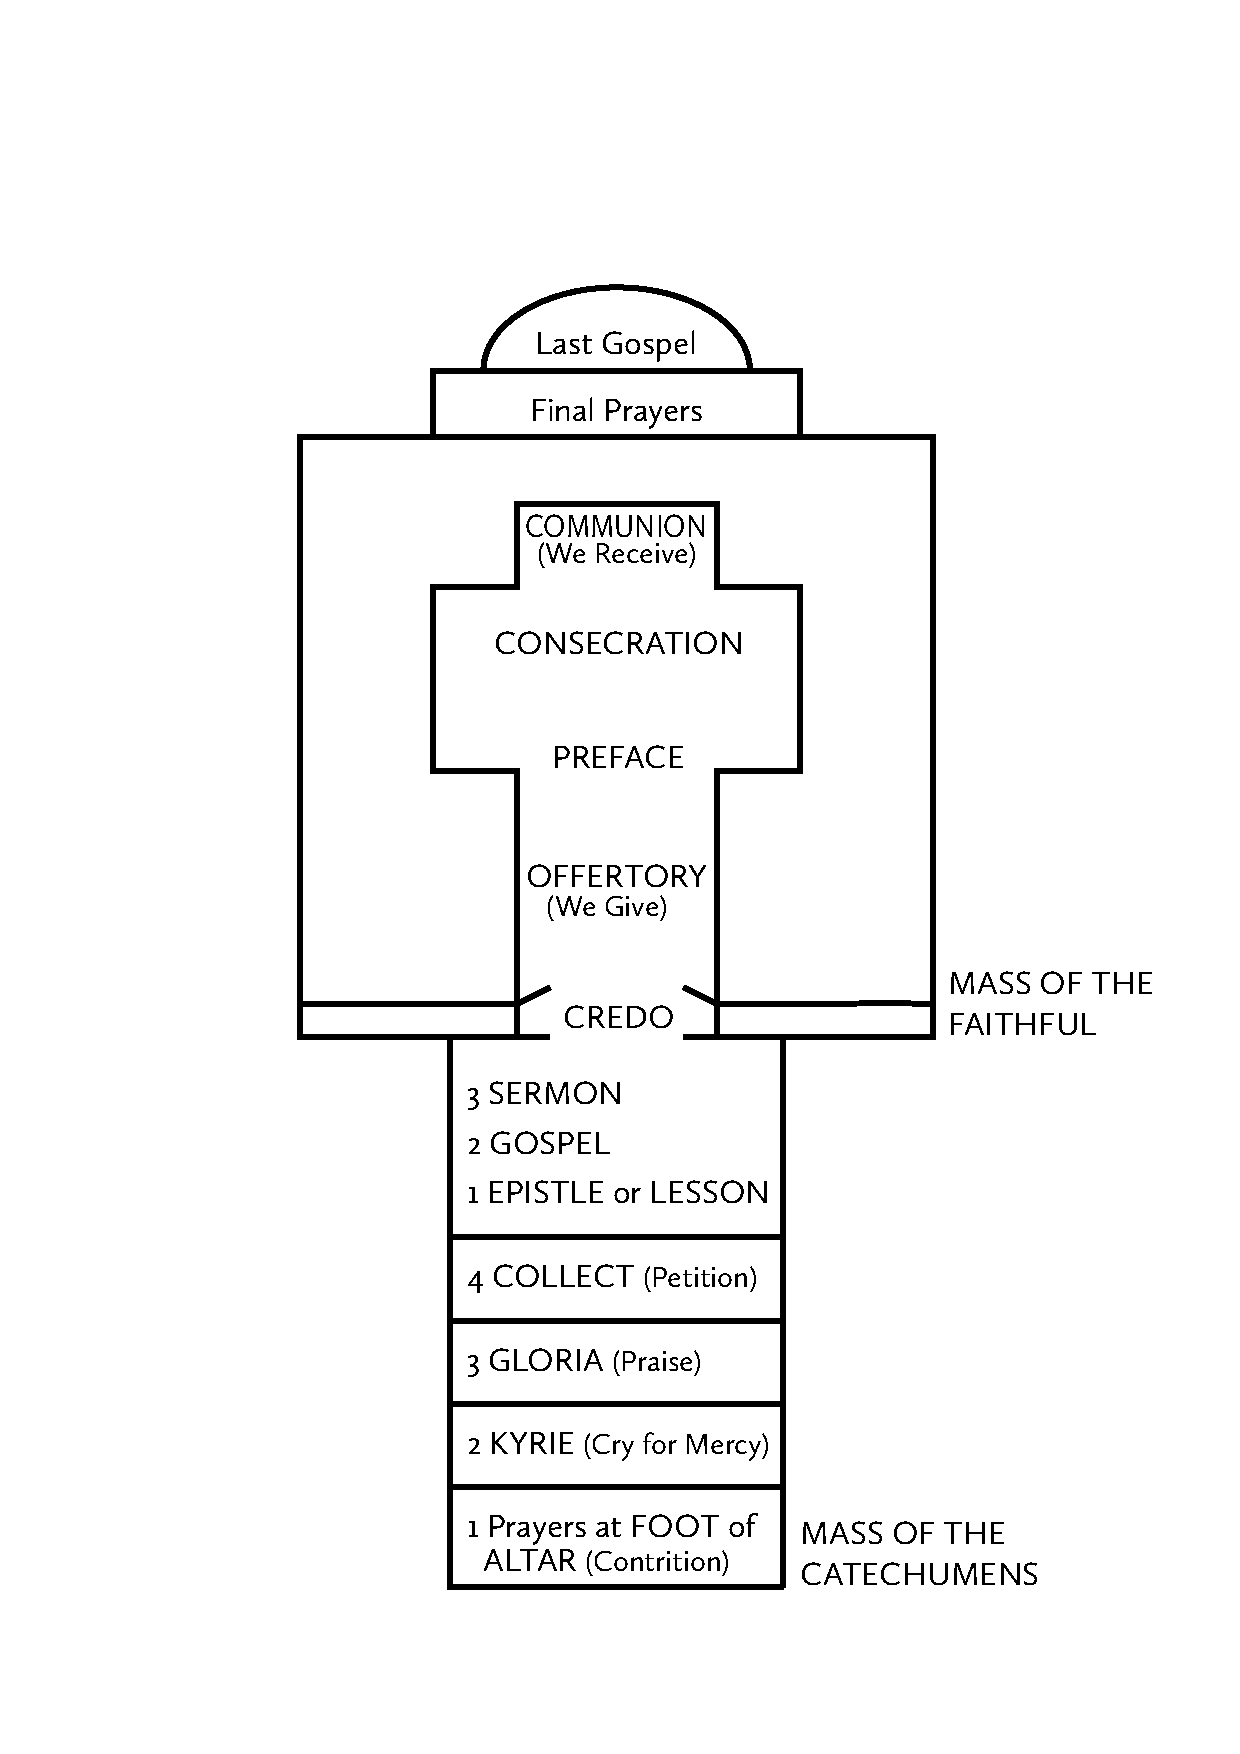
\includegraphics[width=11cm]{images/PLANOFTHEMASS.pdf}}

\section*{Plan of the Mass}

\bigskip
\vfill
\newpage

\section{Mass of the Catechumens}

\rubrics{The choir chants the Introit as the priest begins the opening
prayers quietly with the servers.}

\See{the Introit in the Proper of the Mass, HC p.~\pageref{hc-int}, BVM p.~\pageref{bvm-int}, SSJ p.~\pageref{ssj-int}, CRex p.~\pageref{cr-int}.}

\medskip

\kneel

\let\newtextbf\textbf

\let\textbf\oldtextbf

\begin{Parallel}{\gcolwidth}{\gcolwidth}
\firstlatin{I}{n nomine Patris,}{ \maltese et Fílii, et Spíritus
Sancti.\\ \all{\embolden{Amen.}}}
\firstvern{I}{n the Name of the Father,}{\maltese and of the
Son, and of the Holy Ghost. Amen.}


\latin{\Pnobar Introíbo ad altáre Dei.}
\vern{I will go in unto the Altar of God.}
%
\latin{\all{\embolden{Ad Deum qui l\ae tíficat}\\%
\embolden{juventútem meam.}}}
\vern{To God, who giveth joy to my youth.}
\end{Parallel}

\smallskip

\source{Psalm 42}

%*\small
%\font\gregoriosymbolfont=gresym at \smallR
\smallskip

\begin{Parallel}{\gcolwidth}{\gcolwidth}
\firstlatin{J}{udica}{ me, Deus, et discérne causam meam de gente non sancta;
ab hómine iníquo et dolóso érue me.}
\firstvern{J}{udge}{ me, O God, and distinguish my
cause from the nation that is not holy: deliver me from the unjust
and deceitful man.}
%
\latin{\all{\embolden{Quia tu es, Deus, fortitúdo}\\%
\embolden{mea: quare me repulísti,}\\%
\embolden{et quare tristis incédo,}\\%
\embolden{dum afflígit me inimícus?}}}
\vern{For Thou, O God, art my strength: why hast Thou cast me off? and
why do I go sorrowful whilst the enemy afflicteth me?}
%
\latin{\Pnobar Emítte lucem tuam et veritátem tuam: ipsa me deduxérunt %
et adduxérunt in montem sanctum tuum, et in tabernácula tua.}
\vern{Send forth Thy light and Thy truth: they have led me, and brought %
me unto Thy holy hill, and into Thy tabernacles.}
%
\latin{\all{\embolden{Et introíbo ad altáre Dei:}\\%
\embolden{ad Deum qui l\ae tíficat}\\%
\embolden{juventútem meam.}}}
\vern{And I will go in unto the Altar of God: unto God who giveth joy
to my youth.}
%
\latin{\Pnobar Confitébor tibi in cíthara, Deus, Deus meus: quare
tristis es ánima mea, et quare contúrbas me?}
\vern{I will praise Thee upon the harp, O God, my God: why art thou sad,
O my soul? and why dost thou disquiet me?}
%
\latin{\all{\embolden{Spera in Deo, quóniam adhuc}\\%
\embolden{confitébor illi: salutáre vultus}\\%
\embolden{mei, et Deus meus.}}}
\vern{Hope thou in God, for I will yet praise Him: who is the salvation
of my countenance, and my God.}
%
\latin{\Pnobar Glória Patri, et Fílio, et Spirítui Sancto.}
\vern{Glory be to the Father, and to the Son, and to the Holy Ghost.}
%
\latin{\all{\embolden{Sicut erat in princípio, et}\\
\embolden{nunc, et semper, et in s\'\ae cula}\\
\embolden{s\ae culórum. Amen.}}}
\vern{As it was in the beginning is now, and ever shall be, world without
end. Amen.}

\normalsize%\font\gregoriosymbolfont=gresym at \regularR

\twocolspace{0.4mm}

\latin{\Pnobar Introíbo ad altáre Dei.}
\vern{I will go in unto the Altar of God.}
%
\latin{\all{\embolden{Ad Deum qui l\ae tíficat}\\%
\embolden{juventútem meam.}}}
\vern{To God, who giveth joy to my youth.}

\twocolspace{0.4mm}

\latin{\Vbar Adjutórium nostrum \maltese in nómine Dómini.}
\vern{Our help \maltese is in the Name of the Lord.}

\latin{\all{\embolden{Qui fecit c\ae lum et terram.}\\ \vspace{6pt}}}
\vern{Who hath made heaven and earth.}
\end{Parallel}
\smallskip

\rubrics{Joining his hands humbly bowing down the priest says
the Confiteor.}

\smallskip
\begin{Parallel}{\gcolwidth}{\gcolwidth}
\latin{Confíteor Deo omnipoténti, \&c.}
\vern{I confess to Almighty God, \&c.}

\twocolspace{0.2mm}
\latin{\all{\embolden{Misereátur tui omnípotens}\\%
\embolden{Deus, et dimíssis peccátis tuis,}\\%
\embolden{perdúcat te ad vitam \ae térnam.}}}
\vern{May Almighty God have mercy upon you, forgive you your sins, and
bring you to life everlasting.}



\latin{\Pnobar Amen.}
\vern{Amen.}
\end{Parallel}

\smallskip

\rubrics{The servers say the Confiteor on behalf of those present.}

\smallskip

\begin{Parallel}{\gcolwidth}{\gcolwidth}
\firstlatin{C}{\textbf{onfiteor}}{\textbf{ Deo omnipoténti, %\parfillskip0pt 
beát\ae\ Marí\ae\ semper Vírgini, beáto
Michaéli Archángelo, beáto Joánni Baptíst\ae, sanctis Apóstolis Petro
et Paulo, ómnibus Sanctis, et tibi, Pater: quia peccávi nimis cogitatióne,
verbo et ópere:} \textit{(strike breast three times)} \textbf{mea
culpa, mea culpa, mea máxima culpa. Ideo precor beátam Maríam semper
Vírginem, beátum Michaélem Archángelum, beátum Joánnem Baptístam,
sanctos Apóstolos Petrum et Paulum, omnes Sanctos, et te, Pater, oráre
pro me ad Dóminum Deum nostrum.}}
\firstvern{I}{ confess}{ to Almighty God, to blessed Mary %\parfillskip0pt 
ever Virgin, to blessed Michael the Arch\-angel, to blessed John the
Baptist, to the holy Apostles Peter and Paul, to all the Saints, and
to you, Father, that I have sinned exceedingly, in thought, word,
and deed: \textit{(strike breast three times)} through my fault,
through my fault, through my most grievous fault. Therefore I beseech
blessed Mary ever Virgin, blessed Michael the Arch\-angel, blessed John
the Baptist, the holy Apostles Peter and Paul, all the Saints, and
you, Father, to pray for me to the Lord our God.}
%\latin{}
%\vern{}
\end{Parallel}
\smallskip

%\twocolspace{0.2mm}


\let\textbf\newtextbf

%\let\newtextbf\textbf

%\let\textbf\oldtextbf

\smallskip
\begin{Parallel}{\gcolwidth}{\gcolwidth}
\latin{\Pnobar Misereátur vestri omnípotens Deus, et dimíssis peccátis
vestris, perdúcat vos ad vitam \ae térnam.}
\vern{May Almighty God have mercy upon you, forgive you your sins, and
bring you to life everlasting.}

\latin{\all{Amen.}}
\vern{Amen.}

\twocolspace{0.2mm}

\latin{Indulgéntiam, \maltese absolutiónem, et remissiónem peccatórum
nostrórum, tríbuat nobis omnípotens et miséricors Dóminus.}
\vern{May the Almighty and merciful Lord grant us pardon, \maltese absolution,
and remission of our sins.}

\latin{\all{Amen.}}
\vern{Amen.}

\twocolspace{0.2mm}

\latin{\Vbar Deus, tu convérsus vivificábis nos.}
\vern{Thou wilt turn, O God, and bring us to life.}

\latin{\all{Et plebs tua l\ae tábitur in te.}\\ \ }
\vern{And Thy people shall rejoice in Thee.}

\latin{\Vbar Osténde nobis, Dómine, misericórdiam tuam.}
\vern{Show us, O Lord, Thy mercy.\\ \ }

\latin{\all{Et salutáre tuum da nobis.}}
\vern{And grant us Thy salvation.}

\latin{\Vbar Dómine, exáudi oratiónem me\-am.}
\vern{O Lord, hear my prayer.}

\latin{\all{Et clamor meus ad te véniat.}}
\vern{And let my cry come unto Thee.}

\latin{\Vbar Dóminus vobíscum.}
\vern{The Lord be with you.}

\latin{\all{Et cum spíritu tuo.}}
\vern{And with thy spirit.}

\latin{Orémus.}
\vern{Let us pray.}

\end{Parallel}

\HMstand

%*\small
%\font\gregoriosymbolfont=gresym at \smallR

\smallskip

\rubrics{Then going up the Altar he says silently,}

\smallskip
\begin{Parallel}{\gcolwidth}{\gcolwidth}
\latin{Aufer a
nobis, qu\'\ae sumus, Dómine, iniquitátes nostras: ut ad Sancta sanctórum
puris mereámur méntibus introíre. Per Christum Dó\-mi\-num nostrum. Amen.}
\vern{Take away from us our iniquities, we entreat
Thee, O Lord, that with pure minds we may worthily enter into the
Holy of Holies. Through Christ our Lord. Amen.}
\end{Parallel}
%\bigskip

\rubrics{He kisses the Altar in the middle where the relics
of the Saints are enclosed saying silently,}

\smallskip

\begin{Parallel}{\gcolwidth}{\gcolwidth}
\latin{Orámus te,
Dómine, per mérita Sanctórum tuórum, quorum re\-lí\-qui\ae\ hic sunt,
et ómnium Sanctórum: ut indúlgere dignéris ómnia peccáta mea. Amen.}
\vern{We beseech Thee, O Lord, by the merits of Thy Saints, whose
relics are here, and of all the Saints, that Thou wilt deign to pardon
me all my sins. Amen.}
\end{Parallel}
\smallskip

\rubrics{At a high Mass the priest incenses the Altar, first blessing the incense.}

\smallskip

\begin{Parallel}{\gcolwidth}{\gcolwidth}
\latin{Ab illo \maltese benedicáris, in cujus honóre cremáberis.
Amen.}
\vern{Be blessed \maltese by Him in whose honour thou art burnt. Amen.}
\end{Parallel}

\eject

\rubrics{The priest makes the Sign of the Cross and reads the Introit.}

%\bigskip

\normalsize%\font\gregoriosymbolfont=gresym at \regularR

%\rubrics{The people sing the Kyrie from the Kyriale}

%\smallskip

\begin{Parallel}{\gcolwidth}{\gcolwidth}
\latin{\celebrant{Kýrie eléison.}}
\vern{Lord have mercy.}
\latin{\all{Kýrie eléison.}}
\vern{Lord have mercy.}
\latin{\celebrant{Kýrie eléison.}}
\vern{Lord have mercy.}

\latin{\all{Christe eléison.}}
\vern{Christ have mercy.}
\latin{\celebrant{Christe eléison.}}
\vern{Christ have mercy.}
\latin{\all{Christe eléison.}}
\vern{Christ have mercy.}

\latin{\celebrant{Kýrie eléison.}}
\vern{Lord have mercy.}
\latin{\all{Kýrie eléison.}}
\vern{Lord have mercy.}
\latin{\celebrant{Kýrie eléison.}}
\vern{Lord have mercy.}

\twocolspace{0.5mm}

%\rubrics{At the middle of the Altar, the priest intones the
%Gloria, which the people continue from the Kyriale.}

%\smallskip

\firstlatin{G}{loria}{ in excélsis %\parfillskip0pt
Deo, et in terra pax hóminibus bon\ae\ voluntátis. Laudámus te. Benedícimus te. Adorámus te. Glorificámus te. Grátias
ágimus tibi propter magnam glóriam tuam. Dómine Deus, Rex c\ae léstis,
Deus Pater omnípotens. Dómine Fili unigénite, Jesu Christe. Dómine
Deus, Agnus Dei, Fílius Patris. Qui tollis peccáta mundi, miserére
nobis. Qui tollis peccáta mundi, súscipe deprecatiónem nostram. Qui
sedes ad déxteram Patris, miserére nobis. Quóniam tu solus Sanctus.
Tu solus Dóminus. Tu solus Altíssimus, Jesu Christe. Cum Sancto Spíritu,
\maltese in glória Dei Patris. Amen.}
\firstvern{G}{lory}{ be to God on high. And on earth %\parfillskip0pt 
peace to men of good will. We praise Thee. We bless Thee. We adore Thee.
We glorify Thee. We give Thee thanks for Thy great glory. Lord God,
heavenly King, God the Father Almighty. Lord Jesus Christ, Only-begotten
Son, Lord God, Lamb of God, Son of the Father.  Who takest away
the sins of the world, have mercy on us.  Who takest away the
sins of the world, receive our prayer. Who sittest at the right
hand of the Father, have mercy on us. For Thou alone art holy. Thou
alone art the Lord. Thou alone, O Jesus Christ, art most high. With
the Holy Ghost, \maltese in the glory of God the Father. Amen.}
%\latin{}
%\vern{}
%\latin{}
%\vern{}
\end{Parallel}
\smallskip

\rubrics{He kisses the Altar, and turning toward the people
chants,}

\smallskip
\begin{Parallel}{\gcolwidth}{\gcolwidth}
 \latin{\celebrant{Dóminus vobíscum.}}
 \vern{The Lord be with you.}

 \latin{\all{Et cum spíritu tuo.}}
 \vern{And with thy spirit.}
 
 \latin{\celebrant{Orémus.}}
 \vern{Let us pray.}
\end{Parallel}
\bigskip

\rubrics{He returns to the Missal and chants the Collect.}

\begin{Parallel}{\gcolwidth}{\gcolwidth}
\latin{{\ldots}per ómnia saécula saeculórum.}
\vern{{\ldots}world without end.}
\latin{\all{Amen.}}
\vern{Amen.}
\end{Parallel}

\See{the Collect in the Proper of the Mass, HC p.~\pageref{hc-col}, BVM p.~\pageref{bvm-col}, SSJ p.~\pageref{ssj-col}, CRex p.~\pageref{cr-col}.}

%\bigskip

\subsection*{The Epistle}

\sit

\See{the Epistle in the Proper of the Mass, HC p.~\pageref{hc-ep}, BVM p.~\pageref{bvm-ep}, SSJ p.~\pageref{ssj-ep}, CRex p.~\pageref{cr-ep}.}

\rubrics{Then is read the Epistle for the day.  After which,}

\begin{Parallel}{\gcolwidth}{\gcolwidth}
%\latin{Lectio \ldots}
%\vern{A reading \ldots}
\latin{\all{Deo grátias.}}
\vern{Thanks be to God.}
\end{Parallel}

%\bigskip
%\goodbreak

\rubrics{The priest then reads the Gradual and Alleluia while these are chanted by the choir.}

\See{the Gradual and Alleluia in the Proper of the Mass, HC p.~\pageref{hc-gra}, BVM p.~\pageref{bvm-gra}, SSJ p.~\pageref{ssj-gra}, CRex p.~\pageref{cr-gra}.}

%oo\newpage

\small
%\font\gregoriosymbolfont=gresym at \smallR

\rubrics{At a high Mass the incense is blessed and the Deacon says,}
\smallskip
\begin{Parallel}{\gcolwidth}{\gcolwidth}
\latin{Munda cor meum ac lábia mea, omnípotens Deus, qui lábia Isaí\ae\ prophét\ae\ cálculo
mundásti igníto: ita me tua grata miseratióne dignáre mundáre, ut
sanctum Evangélium tuum digne váleam nuntiáre. Per Christum Dóminum
nostrum. Amen.}
\vern{\tolerance=1000 Cleanse my heart and my lips, O Almighty
God, who didst cleanse the lips of the prophet Isaiah with a burning
coal; through Thy gracious mercy so purify me that I may worthily
proclaim Thy holy Gospel. Through Christ our Lord. Amen.}

\smallskip

\latin{Jube, Dómine, benedícere.}
\vern{Lord, grant Thy blessing.}

\smallskip

\latin{Dóminus sit in corde meo, et in lábiis meis (tuis):
ut digne et competénter annúntiem Evangélium suum.}% In
%nómine Patris, \maltese et Fílii, et Spíritus Sancti. Amen.}
\vern{May the Lord be in my heart and on my lips that I may
worthily and fittingly proclaim His Gospel.}% In the Name
%of the Father, \maltese and of the Son and of the Holy Ghost. Amen.}

\normalsize%\font\gregoriosymbolfont=gresym at \regularR

\twocolspace{0.3mm}

\subsection*{The Gospel}

\stand

 \latin{\celebrant{Dóminus vobíscum.}}
 \vern{The Lord be with you.} 

\latin{\all{Et cum spíritu tuo.}}
\vern{And with thy spirit.}

\latin{\celebrant{Sequéntia sancti Evángelii secúndum N.}}
\vern{The continuation of the holy Gospel according to N.}

\latin{\all{Glória tibi, Dómine.}}
\vern{Glory to Thee, O Lord.}
\end{Parallel}

\normalsize

\rubrics{The priest or deacon chants the Gospel.}

\See{the Gospel in the Proper of the Mass, HC p.~\pageref{hc-gos}, BVM p.~\pageref{bvm-gos}, SSJ p.~\pageref{ssj-gos}, CRex p.~\pageref{cr-gos}.}

\begin{Parallel}{\gcolwidth}{\gcolwidth}
\latin{\all{Laus tibi, Christe.}}
\vern{Praise be to Thee, O Christ.}
\end{Parallel}

\subsection*{The Sermon}

\rubrics{The priest or deacon may give a sermon.}

\sit

\bigskip
%\newpage

\subsection*{The Creed}

\rubrics{The priest returns to the Altar and intones the Credo.}

\stand

\smallskip

\begin{Parallel}{\gcolwidth}{\gcolwidth}
\firstlatin{C}{redo}{ in unum
Deum, Patrem omnipoténtem, factórem c\ae  li et terr\ae ,
visibílium ómnium et invisibílium. Et in unum Dóminum Jesum Christum,
%!\parfillskip0pt
Fílium Dei unigénitum.
Et ex Patre natum ante ómnia s\'\ae  cula. Deum
de Deo, lumen de lúmine, Deum verum de Deo vero. Génitum, non factum,
consubstantiálem Patri: per quem ómnia facta sunt. Qui propter nos
hómines, et propter nostram salútem descéndit de c\ae  lis.}
\firstvern{I}{ believe}{ in one God, the Father Almighty, Maker of heaven and earth, and of all things visible and invisible.
%!\parfillskip0pt
And in one Lord Jesus Christ, the Only-begotten Son of God.
Born of
the Father before all ages. God of God, Light of Light, true God of 
true God. Begotten, not made: consubstantial with the Father; by whom
all things were made. Who for us men, and for our salvation came, down from heaven.}

\rubrics{Here all genuflect.}
%\vskip-6pt
%\phantom{Invisible text}
%\twocolspace{0.2mm}
\smallskip

\goodbreak

\latin{Et incarnátus est de Spíritu Sancto ex María
Virgine: \textsc{et homo factus est}.}
\kneel
\vern{And was incarnate by the Holy Ghost of the Virgin Mary: \textsc{and was made man}.}


\stand
%\twocolspace{0.2mm}
\smallskip

\latin{Crucifíxus étiam pro nobis: sub Póntio Piláto passus,
et sepúltus est. Et resurréxit tértia die, secúndum Scriptúras. Et
ascéndit in c\ae  lum: sedet ad déxteram Patris. Et íterum ventúrus
est cum glória judicáre vivos et mórtuos: cujus regni non erit finis.
Et in Spíritum Sanctum, Dóminum et vivificántem: qui ex Patre, Filióque
procédit. Qui cum Patre, et Fílio simul adorátur et conglorificátur:
qui locútus est per Prophétas. Et unam, sanctam, cathólicam et apostólicam
Ecclésiam. Confíteor unum baptísma in remissiónem peccatórum. Et expécto
resurrectiónem mortuórum. Et vitam \maltese ventúri s\'\ae  culi. Amen.}
\vern{\pretolerance=500 \tolerance=1000 He was also crucified for us, suffered under Pontius Pilate, and was
buried. And on the third day He rose again according to the Scriptures.
And He ascended into heaven and sitteth at the right hand of the Father.
And He shall come again with glory to judge the living and the dead:
of whose kingdom there shall be no end. And in the Holy Ghost, the
Lord and Giver of life: who proceedeth from the Father and the Son.
Who together with the Father and the Son is adored and glorified:
who spoke through the Prophets. And One, Holy, Catholic and Apostolic
Church. I confess one baptism for the remission of sins. And I look
for the resurrection of the dead and the life \maltese of the world to come.
Amen.}
\end{Parallel}

\newpage

\section{Mass of the Faithful}

\begin{Parallel}{\gcolwidth}{\gcolwidth}
\latin{\celebrant{Dóminus vobíscum.}}
\vern{The Lord be with you.}

\latin{\all{Et cum spíritu tuo.}}
\vern{And with thy spirit.}
 
 \latin{\celebrant{Orémus.}}
 \vern{Let us pray.}

\rubrics{The priest reads the Offertory, which is sung by the choir.}

\smallskip

\sit

\See{the Offertory in the Proper of the Mass, HC p.~\pageref{hc-off}, BVM p.~\pageref{bvm-off}, SSJ p.~\pageref{ssj-off}, CRex p.~\pageref{cr-off}.}

%*\small
%\font\gregoriosymbolfont=gresym at \smallR

\latin{Súscipe, sancte
Pater, omnípotens \ae térne Deus, hanc immaculátam
%\parfillskip0pt
hóstiam, quam ego indígnus fámulus tuus óffero tibi Deo meo vivo et
vero, pro innumerabílibus peccátis, et offensiónibus, et negligéntiis
meis, et pro ómnibus circumstántibus, sed et pro ómnibus fidélibus
christiánis vivis atque defúnctis: ut mihi et illis profíciat ad salútem
in vitam \ae térnam. Amen.}
\vern{Accept, O Holy Father, Almighty and Everlasting
%\parfillskip0pt
God, this unspotted Host, which I, Thine unworthy servant, offer unto
Thee, my living and true God, to atone for my countless sins, offences
and negligences: on behalf of all here present and likewise for all
faithful Christians, living and dead, that it may avail both me and
them as a means of salvation, unto life everlasting. Amen.}

%\latin{}
%\vern{}

\rubrics{Making the Sign of the Cross with the paten, he places
the host upon the corporal. The wine and water are poured into the
chalice, the priest blesses the water before it is mixed, saying
silently,}

\smallskip

\latin{\pretolerance=500 \tolerance=1000 Deus,
\maltese qui humán\ae\ substánti\ae\ dignitátem mirabíliter condidísti,
et mirabílius reformásti: da nobis per hujus aqu\ae\ et vini mystérium,
ejus divinitátis esse consórtes, qui humanitátis nostr\ae\ fíeri
dignátus est párticeps, Jesus Christus Fílius tuus Dóminus noster:
Qui tecum vivit et regnat in unitáte Spíritus Sancti Deus: per ómnia
s\'\ae cula s\ae culórum. Amen.}
\vern{O God, \maltese who in creating man didst exalt
his nature very wonderfully and yet more wonderfully didst establish
it anew; by the Mystery signified in the mingling of this water and
wine, grant us to have part in the Godhead of Him who hath deigned
to become a partaker of our humanity, Jesus Christ, Thy Son, our Lord;
who liveth and reigneth with Thee in the unity of the Holy Ghost,
God, for ever and ever. Amen.}

\smallskip

\rubrics{Returning to the middle of the Altar, the priest takes
the chalice and offers it to God, saying silently,}

\smallskip

\latin{Offérimus tibi,
Dómine, cálicem salutáris tuam deprecántes cleméntiam: ut in conspéctu
divín\ae\ majestátis tu\ae, pro nostra et totíus mundi salúte cum
odóre suavitátis ascéndat. Amen.}
\vern{We offer unto Thee, O Lord, the chalice
of salvation, entreating Thy mercy that our offering may ascend with
a sweet fragrance in the sight of Thy divine Majesty, for our own
salvation and for that of the whole world. Amen.}

\smallskip

\rubrics{He makes the Sign of the Cross with the chalice, and
placing it on the corporal, he covers it with the pall. Bowing down,
he says silently,}

\smallskip

\latin{In spíritu humilitátis,
et in ánimo contríto suscipiámur a te, Dómine, et sic fiat sacrifícium
nostrum in conspéctu tuo hódie, ut pláceat tibi, Dómine Deus.}
\vern{Humbled in spirit and contrite of heart,
may we find favour with Thee, O Lord: and may our sacrifice be so
offered this day in Thy sight as to be pleasing to Thee, O Lord God.}

\smallskip

\rubrics{Raising his eyes and extending his hands, he says silently,}

\smallskip

\latin{Veni,
Sanctificátor omnípotens \ae\-tér\-ne Deus: et bénedic \maltese hoc sacrifícium,
tuo sancto nómini pr\ae\-pará\-tum.}
\vern{Come, O Sanctifier, Almighty and
Eternal God, and bless \maltese this sacrifice which is prepared for
the glory of Thy holy Name.}

\smallskip

\small

\rubrics{When the offerings of bread and wine are to be incensed, as well as the altar and all who are present, the priest blesses the incense.\\  Otherwise skip ahead to the \emph{Lavabo.}}

\smallskip

\latin{\pretolerance=500 \tolerance=1000 Per intercessiónem beáti Michaélis Archángeli, stantis
%\parfillskip0pt
a dextris altáris incénsi, et ómnium electórum suórum, incénsum istud
dignétur Dóminus benedícere, \maltese et in odórem suavitátis accípere. Per
Christum Dóminum nostrum. Amen.}
\vern{May the Lord, by the intercession of
%\parfillskip0pt
blessed Michael the Archangel,
who standeth at the right side of the altar of incense, and of all
His Elect, vouchsafe to bless \maltese this incense and receive it as an
odour of sweetness: through Jesus Christ our Lord. Amen.}

%\latin{}
%\vern{}

\smallskip


\rubrics{The priest incenses the bread and wine.}

\smallskip

\latin{Incénsum istud a te benedíctum ascéndat ad te, Dómine:
et descéndat super nos misericórdia tua.}
\vern{May this incense, which Thou hast blessed, O Lord, ascend to Thee,
and may Thy mercy descend upon us.}

\smallskip

\rubrics{Then he incenses the Altar.}

\smallskip

\latin{Dirigátur, Dómine, orátio mea, sicut incénsum in conspéctu
tuo: elevátio mánuum meárum sacrifícium vespertínum.}
\vern{Let my prayer, O Lord, be directed as incense in Thy sight: the lifting
up of my hands as an evening sacrifice.}
\latin{Pone, Dómine, custódiam ori meo, et óstium circumstánti\ae\ lábiis
meis: ut non declínet cor meum in verba malíti\ae , ad excusándas,
excusatiónes in peccáta.}
\vern{Set a watch, O Lord, before my mouth, and a door round about my lips, that my heart may not incline to evil words, to make excuses for sins.}

\smallskip

%oo\newpage

\rubrics{Returning the thurible, the priest says,}

\smallskip

\latin{Accéndat in nobis Dóminus ignem sui amóris, et flammam
\ae térn\ae\ caritátis. Amen.}
\vern{May the Lord enkindle within us the fire of His love, and the flame
of everlasting charity. Amen.}

\bigskip

\normalsize%\font\gregoriosymbolfont=gresym at \regularR

\rubrics{At a High Mass the priest is now incensed followed by the clergy and then
the people who stand and bow to the thurifer.}

\smallskip

%*\small
%\font\gregoriosymbolfont=gresym at \smallR

\normalsize

\rubrics{He then goes to wash his fingers while he says Psalm
25 6--12 silently,}

\smallskip

\firstlatin{L}{avábo}{ inter
innocéntes manus meas: et circumdábo altáre tuum, Dómine. }
\firstvern{I}{ will}{ wash my hands among the innocent,
and I will encompass Thine altar, O Lord.}

\latin{Ut áudiam
vocem laudis: et enárrem univérsa mirabíla tua.}
\vern{That I may hear the voice
of praise, and tell of all Thy wondrous works.}

\latin{Dómine, diléxi decórem
domus tu\ae : et locum habitatiónis glóriae tu\ae .}
\vern{I have loved, O Lord,
the beauty of Thy house, and the place where Thy glory dwelleth. }

\latin{Ne perdas cum
ímpiis, Deus ánimam meam: et cum viris sánguinum vitam meam. }
\vern{Take
not away my soul, O God, with the wicked, nor my life with men of
blood. }

\latin{In quorum
mánibus iniquitátes sunt: déxtera eórum repléta est munéribus. }
\vern{In whose hands are iniquities, their right hand is filled with
gifts. }

\latin{Ego
autem in innocéntia mea ingréssus sum: rédime me, et miserére mei.}
\vern{But as for me, I have walked in my innocence; redeem me, and
have mercy on me. }

\latin{Pes meus stetit in dirécto: in ecclésiis benedícam te, Dómine. }
\vern{My foot hath stood in the right way; in the churches
I will bless Thee, O Lord. }

\latin{Glória Patri.}
\vern{Glory be.}
%Patri, et Filio, et Spiritui Sancto.}
%\vern{Glory be to the Father, and to the Son,
%and to the Holy Ghost.} 

%\latin{Sicut erat in principio, et nunc,
%et semper, et in s\'\ae cula s\ae culorum. Amen.}
%\vern{As it was in the beginning, is now, and ever
%shall be, world without end. Amen.}

\smallskip

\rubrics{Bowing down before the middle of the Altar, he joins
his hands, saying silently,}

\smallskip

\latin{Súscipe, sancta
Trínitas, hanc oblatiónem, quam tibi offérimus ob
memóriam passiónis, resurrectiónis, et ascensiónis Jesu Christi, Dómini
nostri: et in honórem beát\ae\ Marí\ae\ semper Vírginis, et beáti
Joánnis Baptíst\ae, et sanctórum Apostolórum Petri et Pauli, et istórum,
et ómnium Sanctórum: ut illis profíciat ad honórem, nobis autem ad
salútem: et illi pro nobis intercédere dignéntur in c\ae lis, quorum
memóriam ágimus in terris. Per eúmdem Christum Dóminum nostrum. Amen.}
\vern{Receive, O Holy Trinity, this oblation
which we make to Thee in memory of the Passion, Resurrection, and
Ascension of our Lord Jesus Christ; and in honour of blessed Mary
ever Virgin, of blessed John the Baptist, the holy Apostles Peter
and Paul, of these and of all the Saints. To them let it bring honour,
and to us salvation, and may they whom we are commemorating here on
earth deign to plead for us in heaven. Through the same Christ our
Lord. Amen.}

\bigskip
%\goodbreak

 \normalsize%\font\gregoriosymbolfont=gresym at \regularR

 \rubrics{He kisses the Altar then turns
 and says the first two words aloud and then faces the Altar while concluding
 the prayer silently,}

\smallskip

 \firstlatin{O}{rate fratres:}{ ut meum ac vestrum sacrifícium acceptábile fiat apud Deum Patrem 
 omnipoténtem.}
\firstvern{P}{ray brethren,}{ that my Sacrifice and yours
 may be acceptable to God the Father Almighty.}

\smallskip

\rubrics{The server responds,}

\let\newtextbf\textbf

\let\textbf\oldtextbf


 \latin{\all{\embolden{Suscípiat Dóminus sacrifícium}\\%
\embolden{de mánibus tuis ad laudem}\\%
\embolden{et glóriam nóminis sui,}\\%
\embolden{ad utilitátem quoque nostram,}\\%
\embolden{totiúsque Ecclési\ae\ su\ae\ sanct\ae.}}}
 \vern{May the Lord accept the Sacrifice from thy hands, to the praise
 and glory of His Name, for our benefit and for that of all His holy
 Church.}

\let\textbf\newtextbf


\bigskip

\rubrics{Then with outstretched hands, the priest says the Secret in silence.}

\See{the Secret in the Proper of the Mass, HC p.~\pageref{hc-sec}, BVM p.~\pageref{bvm-sec}, SSJ p.~\pageref{ssj-sec}, CRex p.~\pageref{cr-sec}.}

%\includescore{kyriale/prepref.tex}

\latin{{\ldots}per ómnia saécula saeculórum.}
\vern{{\ldots}world without end.}
\latin{\all{Amen.}}
\vern{Amen.}
\HMstand
\latin{\celebrant{Dóminus vobíscum.}}
\vern{The Lord be with you.}
\latin{\all{Et cum spíritu tuo.}}
\vern{And with thy spirit.}
\latin{\celebrant{Sursum corda.}}
\vern{Let us lift up our hearts.}
\latin{\all{Habémus ad Dóminum.}}
\vern{We do lift them up to the Lord.}
\latin{\celebrant{Grátias agámus Dómino Deo nostro.}}
\vern{Let us give thanks to the Lord our God.}
\latin{\all{Dignum et justum est.}}
\vern{It is fitting and just.}

\bigskip

\subsection*{The Preface}

\rubrics{With hands extended, the priest chants the Preface.  The Preface of the Holy Trinity follows which is used on Sundays where there is no preface proper to the feast.}

\See{the Preface in the Proper of the Mass, HC p.~\pageref{hc-pre}, BVM p.~\pageref{bvm-pre}, SSJ p.~\pageref{ssj-pre}, CRex p.~\pageref{cr-pre}.}

\smallskip

\firstlatin{V}{ere}{ dignum
et justum est, \ae\-qu\-um et salutáre, nos tibi semper,
%!\parfillskip0pt 
et ubíque grátias ágere: Dómine sancte, Pater omnípotens, \ae térne
Deus: Qui cum unigénito Fílio tuo, et Spíritu Sancto, unus es Deus,
unus es Dóminus: non in uníus singularitáte persón\ae , sed in uníus
Trinitáte substánti\ae . Quod enim de tua glória, revelánte te, crédimus,
hoc de Fílio tuo, hoc de Spíritu Sancto, sine differéntia discretiónis
%\parfillskip0pt
sentímus. Ut in confessióne ver\ae , sempitérn\ae  que Deitátis,
et in persónis propríetas, et in esséntia únitas, et in majestáte
adorétur \ae  quálitas. Quam laudant Angeli atque Archángeli, Chérubim
quoque ac
Séraphim: qui non cessant clamáre quotídie, una voce dicéntes:}
\firstvern{I}{t is}{ truly fitting and just, right and profitable
%!\parfillskip0pt 
for our salvation, that we should at all times and in all places give
thanks unto Thee, O holy Lord, Father Almighty, Everlasting God; who,
together with Thine only-begotten Son, and the Holy Ghost, art one
God, one Lord: not in the oneness of a single Person, but in the Trinity
of one substance. For what we believe by Thy revelation of Thy glory,
the same do we believe of Thy Son, the same of the Holy Ghost, without
difference or separation. So that in confessing the true and everlasting
%\parfillskip0pt
Godhead, we shall adore distinction in persons, unity in essence,
and equality in majesty. Which the Angels and Archangels, the Cherubim also and 
Seraphim do praise nor cease to cry out as with one voice:}

%\lateng{0mm}{Seraphim: qui non cessant clamare quotidie, una voce dicentes:}
%{Seraphim do praise nor cease to cry out as with one voice:}

\smallskip

%\rubrics{Bells are rung as the people sing the Sanctus from the Kyriale.}
\threebell

\kneel

\smallskip

\firstlatin{S}{anctus,}{ Sanctus,
Sanctus, Dó\-minus Deus Sábaoth. Pleni sunt c\ae li
et terra glória tua. Hosánna in excélsis. \maltese Benedíctus qui venit in
nómine Dómini. Ho\-sánna in excélsis.}
\firstvern{H}{oly,}{ Holy, Holy, Lord God of Hosts. Heaven
and earth are full of Thy glory. Hosanna in the highest. \maltese Blessed
is He who cometh in the Name of the Lord. Hosanna in the highest.}

\end{Parallel}


\bigskip

\newpage

\section*{The Canon of the Mass}

%\centerline{\epsfxsize=55mm \epsfbox{bythecross.eps}}
%\begin{center}
%\includegraphics[width=55mm]{bythecross}
%\end{center}

%*\small
%\font\gregoriosymbolfont=gresym at \smallR

\rubrics{(said quietly by the priest.)}


\smallskip
\begin{Parallel}{\gcolwidth}{\gcolwidth}
%\noindent\begin{minipage}[t]{0.48\columnwidth}%
\firstlatincludge{T}{e igitur,}{ clementíssime Pater, 
%!\parfillskip0pt
per Jesum Christum Fílium tuum, Dóminum nostrum,
súpplices rogámus, ac pétimus, uti accépta hábeas, et benedícas, h\ae c
\maltese dona, h\ae c \maltese múnera, h\ae c \maltese sancta sacrifícia illibáta, in
primis, qu\ae\ tibi offérimus pro Ecclésia tua sancta cathólica:
quam pacificáre, custodíre, adunáre, et régere dignéris toto orbe
terrárum: una cum fámulo tuo Papa nostro N.\ et Antístite nostro N.\ et
ómnibus orthodóxis, atque cathólic\ae\ et apostólic\ae\ fídei cultóribus.\\\strut}
\firstverncludge{M}{ost}{ merciful Father, we humbly pray and
%!\parfillskip0pt
beseech Thee, through Jesus Christ Thy Son, our Lord, to accept and
bless these \maltese gifts, these \maltese presents, these \maltese holy unspotted Sacrifices,
which we offer up to Thee, in the first place, for Thy Holy Catholic
Church, that it may please Thee to grant her peace, to preserve, unite,
and govern her throughout the world; as also for Thy servant N.\ our
Pope, and N.\ our bishop, and for all orthodox believers and all who
profess the Catholic and Apostolic faith.}

\smallskip

%\bigskip

\latin{Meménto, Dómine,
famulórum, famularúmque tuárum N.\ et N.\ et ómnium circumstántium,
quorum tibi fides cógnita est, et nota devótio, pro quibus tibi offérimus:
vel qui tibi ófferunt hoc sacrifícium laudis, pro se, suísque ómnibus:
pro redemptióne animárum suárum, pro spe salútis, et incolumitátis su\ae:
tibíque reddunt vota sua \ae térno Deo, vivo et vero.}
\vern{Be mindful, O Lord, of Thy servants and
handmaids N.\ and N.\ and of all here present, whose faith and devotion
are known to Thee, for whom we offer, or who offer up to Thee, this
Sacrifice of praise for themselves and all those dear to them, for
the redemption of their souls and the hope of their safety and salvation:
who now pay their vows to Thee, the everlasting, living and true God.}

\smallskip

%\bigskip

\latin{Communicántes,
et memóriam venerántes, in primis gloriós\ae\ semper Vírginis Marí\ae,
Genitrícis Dei et Dómini nostri Jesu Christi: sed et beáti Joseph
ejúsdem Vírginis Sponsi, et beatórum Apostolórum ac Mártyrum tuórum,
%\parfillskip0pt
Petri et Pauli, André\ae, Jacóbi, Joánnis, Thom\ae, Jacóbi, Phílippi,
Bartholom\'\ae i, Mat\-th\'\ae i, Simónis, et Thadd\'\ae i: Lini, Cleti,
Cleméntis, Xysti, Cornélii, Cypriáni, Lauréntii, Chrysógoni, Joánnis
et Pauli, Cosm\ae\ et Damiáni: et ómnium Sanctórum tuórum; quorum
méritis precibúsque concédas, ut in ómnibus protectiónis tu\ae\ muniámur
auxílio. Per eúmdem Christum Dóminum nostrum. Amen.}
\vern{\tolerance=1000 In communion with, and honouring the memory
in the first place of the glorious ever Virgin Mary Mother of our
God and Lord Jesus Christ; also blessed Joseph, her Spouse; and likewise
of Thy blessed Apostles and Martyrs, Peter and Paul, Andrew, James,
%\parfillskip0pt
John, Thomas, James, Philip, Bar\-tho\-lo\-mew, Matthew, Simon and Thaddeus,
Linus, Cletus, Clement, Sixtus, Cornelius, Cyprian, Lawrence,
Chrysogonus, John and Paul, Cosmas and Damian, and of all thy Saints. Grant for
the sake of their merits and prayers that in all things we may be
guarded and helped by Thy protection. Through the same Christ our
Lord. Amen.}

\smallskip

%\latin{}
%\vern{}


%\bigskip

%\textsf{\textsc{\small  oblation of the victim to god}}

%\rightline{\epsfxsize=8mm \epsfbox{bell.eps}}
%\rightline{
\includegraphics[width=8mm]{bell}}
%\vskip-8mm
\rubrics{A bell is rung to say that the consecration approaches.}
\ringbell
\smallskip

\firstlatin{H}{anc igitur}{ oblatiónem ser\-vitútis nostr\ae, sed et cunct\ae\ famíli\ae\ tu\ae,
qu\'\ae sumus, Dómine, ut placátus accípias: diésque nostros in tua
pace dispónas, atque ab \ae térna damnatióne nos éripi, et in electórum
tuórum júbeas grege numerári. Per Christum Dóminum nostrum. Amen.}
\firstvern{O}{ Lord,}{ we beseech Thee graciously to accept
this oblation of our service and that of Thy whole household. Order
our days in Thy peace, and command that we be rescued from eternal
damnation and numbered in the flock of Thine elect. Through Christ
our Lord. Amen.}

\smallskip

\latin{Quam oblatiónem
tu, Deus, in ómnibus, qu\'\ae\-sumus, benedíc\-tam, \maltese adscríptam, \maltese
ratam, \maltese rationábilem, acceptabilémque fá\-cere dignéris: ut
nobis Corpus, \maltese 
et Sanguis \maltese fiat dilectíssimi Fílii tui Dómini nostri Jesu
Christi. }%
\vern{Humbly we pray Thee, O God, be pleased
to make this same offering wholly blessed \maltese , to consecrate \maltese it and
approve \maltese it, making it reasonable and acceptable, that it may become
for us the Body \maltese and Blood \maltese of Thy dearly beloved Son, our Lord
Jesus Christ.}

\smallskip

%\textsf{\textsc{  consecration of the host}}

\latin{Qui prídie quam paterétur, accépit panem in sanctas
ac venerábiles manus suas, et elevátis óculis in c\ae lum ad te Deum,
Patrem suum omnipoténtem, tibi grátias agens, benedíxit, \maltese fregit,
dedítque discípulis suis, dicens: Accípite, et manducáte ex hoc omnes.}
\vern{Who, the day before He suffered, took bread into His Holy and venerable
hands, and having lifted His eyes to heaven, to Thee, God, His Almighty
Father, giving thanks to Thee, blessed it, \maltese broke it, and gave it
to His disciples, saying: Take and eat ye all of this.}

\bigskip

\latin{\centerline{\textsc{Hoc est enim Corpus Meum.}}}
\vern{\centerline{\textsc{For this is My Body.}}}

\smallskip


\rubrics{The priest genuflects, elevates the Sacred Host and
genuflects again. \\ Bells are rung thrice.}
\threebell

%\rightline{\epsfxsize=8mm \epsfbox{bell.eps} 
%\epsfxsize=8mm \epsfbox{bell.eps} 
%\epsfxsize=8mm \epsfbox{bell.eps}}
%\rightline{
\includegraphics[width=8mm]{bell}
%
\includegraphics[width=8mm]{bell}
%
\includegraphics[width=8mm]{bell}}

%\textsf{\textsc{\small consecration of the wine}}{\small \par}

\centerline{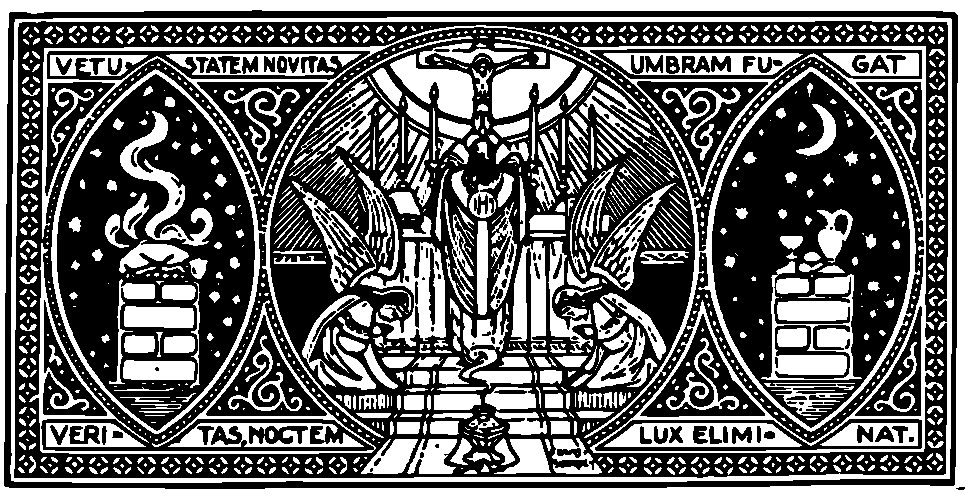
\includegraphics[width=\textwidth]{images/themass14.pdf}}

%\eject

\latin{Símili modo postquam coenátum est, accípiens et hunc
pr\ae clárum Cálicem in sanctas ac venerábiles manus suas: item tibi
grátias agens, benedíxit, \maltese dedítque discípulis suis, dicens: Accépite,
et bíbite ex eo omnes.}
\vern{In like manner, after He had supped, taking also into His holy and
venerable hands this goodly chalice, giving thanks to Thee, He blessed
it, \maltese and gave it to His disciples, saying: Take and drink ye all
of this.}

\medskip

{\tabskip=1em plus2em minus.5em
\halign to\hsize{\hfil\scshape#\hfil&\quad\hfil\scshape#\hfil\cr
  Hic est enim Calix & For this is the Chalice \cr
Sanguinis Mei, novi et & of My Blood, of the new and\cr
\ae terni testamenti: & eternal testament: \cr
mysterium fidei: & the mystery of faith:  \cr
qui pro vobis et & it will be shed for you \cr
pro multis effundetur in & and for many unto  \cr
remissionem peccatorum. & the remission of sins. \cr}}

\bigskip


\latin{H\ae c quotiescúmque fecéritis, in mei memóriam faciétis.}
\vern{As often as ye shall do these 
things, ye shall do them in 
remembrance of Me.}

\bigskip

\rubrics{The priest genuflects, elevates the Chalice and genuflects
again.  Bells are rung thrice.}

%\rightline{\epsfxsize=8mm \epsfbox{bell.eps} 
%\epsfxsize=8mm \epsfbox{bell.eps}
%\epsfxsize=8mm \epsfbox{bell.eps}}
%\rightline{
\includegraphics[width=8mm]{bell}
%
\includegraphics[width=8mm]{bell}
%
\includegraphics[width=8mm]{bell}}
\threebell

%\textsf{\textsc{\small to offer the victim}}{\small \par}

\smallskip


\latin{Unde et
mémores, Dómine, nos servi tui, sed et plebs tua sancta, ejúsdem Christi
Fílii tui Dómini nostri tam beát\ae\ Passiónis, nec non et ab ínferis
Resurrectiónis, sed et in c\ae los gloriós\ae\ ascensiónis: offérimus
pr\ae clár\ae\ majestáti tu\ae\ de tuis donis ac datis hóstiam
\maltese puram, hóstiam \maltese sanctam, hóstiam \maltese immaculátam, Panem \maltese sanctum
vit\ae\ aetérn\ae , et Cálicem \maltese salútis perpétu\ae .}
\vern{And now, O Lord, we, Thy servants, and
with us all Thy holy people, calling to mind the blessed Passion of
this same Christ, Thy Son, our Lord, likewise His Resurrection from
the grave, and also His glorious Ascension into heaven, do offer unto
Thy most sovereign Majesty out of the gifts Thou hast bestowed upon
%us, a Victim \maltese which is pure, a Victim \maltese which is holy, a Victim \maltese\ which is spotless, 
us, a pure \maltese Victim, a holy \maltese Victim, a spotless \maltese\ Victim, 
the holy Bread \maltese of life eternal, and the Chalice
\maltese of everlasting Salvation.}

%\bigskip

\smallskip


%\vspace*{\smallskipamount}
%\textsf{\textsc{\small to ask god to accept our offering}}{\small \par}

\latin{Supra qu\ae \ propítio
ac seréno vultu respícere dignéris; et accépta habére, sicúti accépta
habére dignátus es múnera púeri tui justi Abel, et sacrifícium Patriárch\ae \ nostri
Abrah\ae , et quod tibi óbtulit summus sacérdos tuus Melchísedech,
sanctum sacrifícium, immaculátam hóstiam.}
\vern{Deign to look upon them with a favourable
and gracious countenance, and to accept them as Thou didst accept
the offerings of Thy just servant Abel, and the sacrifice of our Patriarch
Abraham, and that which Thy high priest Melchisedech offered up to
Thee, a holy Sacrifice, an immaculate victim.}


%\bigskip

\smallskip



\latin{Súpplices te
rogámus, omnípotens Deus, jube h\ae c perférri per manus sancti Angeli
tui in sublíme altáre tuum, in conspéctu divín\ae \ majestátis tu\ae :
ut quoquot ex hac altáris participatióne, sacrosánctum Fílii tui Corpus, \maltese
et Sánguinem \maltese sumpsérimus, omni benedictióne c\ae lésti et grátia
repleámur. Per eúmdem Christum Dóminum nostrum. Amen.}
\vern{Humbly we beseech Thee, almighty God, to
command that these our offerings be carried by the hands of Thy holy
Angel to Thine Altar on high, in the sight of Thy divine Majesty,
so that those of us who shall receive the most sacred Body \maltese and Blood
\maltese of Thy Son by partaking thereof from this Altar may be filled with
every grace and heavenly blessing: Through Christ our Lord. Amen.}

%\bigskip


\smallskip

%\textsf{\textsc{\small for the dead}}{\small \par}


\latin{Meménto étiam,
 Dómine, famulórum famularúmque tuárum N.\ et N.\ qui
nos pr\ae cessérunt cum signo fídei, et dórmiunt in somno pacis.}
\vern{Be mindful, also, O Lord, of Thy servants
and handmaids N.\ and N.\ who are gone before us with the sign of
faith and who sleep the sleep of peace.}

%\bigskip

\smallskip

\latin{Ipsis, Dómine, et ómnibus in Christo quiescéntibus, locum refrigérii,
lucis et pacis, ut indúlgeas, deprecámur. Per eúmdem Christum Dóminum
nostrum. Amen.}
\vern{To these, O Lord, and to all
who rest in Christ, grant, we beseech Thee, a place of refreshment,
light, and peace. Through the same Christ our Lord. Amen.}

%\bigskip

\smallskip


%\textsf{\textsc{\small for eternal happiness}} \textsf{\small }{\small \par}

\latin{\textsc{Nobis quoque peccatoribus}  fámulis
tuis, de multitúdine miseratiónum tuárum sperántibus, partem áliquam,
et societátem do\-náre di\-gnéris, cum tuis sanctis Apóstolis et Martýribus,
cum Joánne, Stéphano, Mat\-thía, Bárnaba, Ignátio, Alex\-ándro, Marcellíno,
%\parfillskip0pt
Petro, Felicitáte, Perpétua, Agatha, Lúcia, Agnéte, C\ae cília, Anastásia,
et ómnibus Sanctis tuis, intra quorum nos consórtium, non \ae stimátor
mériti sed véni\ae , qu\'\ae sumus, largítor admítte. Per Christum
Dóminum nostrum.}
\vern{\tolerance=1000 To us also Thy sinful servants, who put our trust in the
multitude of Thy mercies, vouchsafe to grant some part and fellowship
with Thy Holy Apostles and Martyrs: with John, Stephen, Matthias,
Barnabas, Ignatius, Alexander, Marcellinus, Peter, Felicity, Perpetua,
%\parfillskip0pt
Agatha, Lucy, Agnes, Cecilia, Anastasia, and all Thy Saints. Into
their company we beseech Thee admit us, not considering our merits,
but freely %granting us pardon.
pardoning our offenses. 
Through Christ our Lord.}


%\latin{}
%\vern{}

%\bigskip

\smallskip


\latin{Per quem
h\ae c ómnia Dómine, semper bona creas,  sanctíficas,  \maltese vivíficas,  \maltese benedícis, \maltese 
et pr\ae stas nobis.}
\vern{By whom, O Lord, Thou dost always create,
sanctify, \maltese quicken, \maltese bless, \maltese and bestow upon us all these good
things.}

\bigskip


%\textsf{\textsc{\small doxology and minor elevation}}{\small \par}

\latin{\textsc{Per Ipsum,  \maltese et cum Ipso,  \maltese et in Ipso, \maltese}
est tibi Deo Patri \maltese omnipoténti, in unitáte Spíritus \maltese Sancti, omnis
honor et glória,}
\vern{\textsc{Through Him, \maltese and with Him, \maltese and in Him,} \maltese is unto Thee,
God the Father \maltese Almighty, in the unity of the Holy \maltese Ghost, all honour
and glory,}

\bigskip

\normalsize%\font\gregoriosymbolfont=gresym at \regularR

\HMstand

\rubrics{The priest concludes aloud,}
\smallskip

%\includescore{prepater}

\latin{{\ldots}per ómnia saécula saeculórum.}
\vern{{\ldots}world without end.}
\latin{\all{Amen.}}
\vern{Amen.}

\bigskip

\latin{Orémus.}
\vern{Let us pray.}

\latin{Pr\ae céptis salutáribus móniti, et divína
institutióne formáti, audémus dícere:}
\vern{Taught by our Saviour's command and formed by the word
of God, we dare to say:}

\bigskip

\rubrics{The priest continues alone,}
\smallskip

\firstlatin{P}{ater noster,}{ qui es in c\ae lis, sanctificétur nomen tuum: advéniat
regnum tuum: fiat volúntas tua, sicut in c\ae lo, et in terra. Panem
nostrum quotidiánum da nobis hódie, et dimítte nobis débita nostra,
sicut et nos dimíttimus debitóribus nostris.
Et ne nos indúcas in tentatiónem.}
\firstvern{O}{ur Father,}{ who art in heaven, hallowed
be Thy Name; Thy Kingdom come; Thy will be done on earth as it is
in heaven, Give us this day our daily bread; and forgive us our trespasses
as we forgive those who trespass against us. And lead us not into temptation.}


\bigskip

\latin{\all{Sed líbera nos a malo.}}
\vern{But deliver us from evil.}

%\bigskip

%*\small
%\font\gregoriosymbolfont=gresym at \smallR

\rubrics{The priest says silently,} 
\latin{Amen.}
\vern{Amen.}

\medskip

\firstlatin{L}{ibera nos,}{ qu\'\ae sumus, Dó\-mine, ab ómnibus malis, %!\parfillskip=0pt 
pr\ae\-terítis, pr\ae\-séntibus, et futúris, et intercedénte beáta et gloriósa semper Vírgine Dei Genitríce
María, cum beátis Apóstolis tuis Petro et Paulo, atque Andréa, et
ómnibus Sanctis, \maltese da propítius pacem in diébus nostris, ut ope misericórdi\ae\ tu\ae\ adjúti,
et a peccáto simus semper líberi, et ab omni perturbatióne secúri.}
\firstvern{D}{eliver us,}{ we beseech Thee, O Lord, from %!\parfillskip=0pt
all evils, past, present, and to come; and by the intercession of
the blessed and glorious Mary, ever Virgin, Mother of God, together
with Thy blessed Apostles Peter and Paul, and Andrew, and all the
Saints, \maltese mercifully grant us peace in our days, that through the
bounteous help of Thy mercy, we may be always free from sin and safe
from all disquiet.}

\rubrics{The priest breaks the Sacred Host in two.  He places one half on the paten and breaks off a particle from the other.}

\latin{Per eúndem Dóminum nostrum Jesum Christum Fílium tuum,
 Qui tecum vivit et regnat in unitáte Spíritus Sancti
Deus, \ldots}
\vern{Through the same Jesus Christ, Thy Son, our Lord,
who liveth and reigneth with Thee in the unity of the Holy Ghost,
God, \ldots}

%\smallskip
%\normalsize%\font\gregoriosymbolfont=gresym at \regularR
\rubrics{The priest concludes aloud,}

\latin{\ldots{}per ómnia saécula saeculórum.}
\vern{\ldots{}world without end.}
\latin{\all{Amen.}}
\vern{Amen.}
\latin{\celebrant{Pax Dómini sit semper vo\-bís\-cum.}}
\vern{The peace of the Lord be with you always.}
\latin{\all{Et cum spíritu tuo.}}
\vern{And with thy spirit.}

%\bigskip

%*\small
%\font\gregoriosymbolfont=gresym at \smallR

\rubrics{The priest puts the particle into the chalice saying in a low voice,}

\latin{Haec commíxtio et consecrátio Córporis et Sánguinis Dómini
nostri Jesu Christ fiat accipiéntibus nobis in vitam aetérnam. Amen.}
\vern{May this mixture and consecration of the Body and Blood of our
Lord Jesus Christ be to us that receive it effectual to eternal life.
Amen.}

\rubrics{Striking his breast three times, the priest says aloud,}

\normalsize%\font\gregoriosymbolfont=gresym at \regularR

%\rubrics{The people sing the Agnus Dei from the Kyriale}

%\subsection*{The Agnus Dei}

 \smallskip
 
 \kneel

\firstlatin{A}{gnus}{ Dei, qui tollis peccáta mundi, miserére nobis.}
\firstvern{L}{amb}{ of God, who takest away the sins of the world, have mercy on us.}

\latin{Agnus Dei, qui tollis peccáta mundi, miserére nobis.}
\vern{Lamb of God, who takest away the sins of the world, have mercy on us.}

\latin{Agnus Dei, qui tollis peccáta mundi, dona nobis pacem.}
\vern{Lamb of God, who takest away the sins of the world, grant us peace.}
%\end{Parallel}
%\bigskip

%*\small
%\font\gregoriosymbolfont=gresym at \smallR


\rubrics{With his eyes directed toward the Sacrament, he says
silently,}
\smallskip

\latin{Dómine Jesu
Christe, qui dixísti Apóstolis tuis: Pacem relínquo vobis, pacem meam
do vobis: ne respícias peccáta mea, sed fidem Ecclési\ae\ tu\ae :
eámque secúndum voluntátem tuam pacificáre et coadunáre dignéris:
Qui vivis et regnas Deus per ómnia s\'\ae cula s\ae culórum. Amen.}
\vern{O Lord, Jesus Christ, who didst say to
Thine Apostles: Peace I leave you, My peace I give you: look not upon
my sins, but upon the faith of Thy Church; and deign to give her that
peace and unity which is agreeable to Thy will: God who livest and
reignest world without end. Amen.}


\rubrics{At a Solemn Mass, the Kiss of Peace is given to the
Deacon,}
%\smallskip


 \latin{\Vbar Pax tecum.}
\vern{Peace be with thee.} 

 %\smallskip

 \latin{\all{Et cum spíritu tuo.}}
\vern{And with thy spirit.}

%\medskip

%\rubrics{The priest then continues silently,}
\smallskip

\latin{Dómine Jesu
Christe, Fili Dei vivi, qui ex voluntáte Patris, cooperánte Spíritu
Sancto, per mortem tuam mundum vivificásti: líbera me per hoc sacrosánctum
Corpus et Sánguinem tuum ab ómnibus iniquitátibus meis, et univérsis
malis: et fac me tuis semper inh\ae rére mandátis, et a te numquam
separári permíttas: Qui cum eódem Deo Patre, et Spíritu Sancto vivis
et regnas Deus in s\'\ae cula s\ae culórum. Amen.}
\vern{O Lord Jesus Christ, Son of the living
God, who, by the will of the Father and the co-operation of the Holy
Ghost, hast by Thy death given life to the world: deliver me by this,
Thy most sacred Body and Blood, from all my iniquities and from every
evil; make me cling always to Thy commandments, and permit me never
to be separated from Thee. Who with the same God, the Father and the
Holy Ghost, livest and reignest God, world without end. Amen.}

\smallskip

\latin{Percéptio,
Córporis tui, Dómine Jesu Christe, quod ego indígnus súmere pr\'\ae sumo, 
non mihi provéniat in judícium et condemnatiónem: sed pro tua
pietáte, prosit mihi ad tutaméntum mentis et córporis, et ad medélam
percipiéndam. Qui vivis et regnas cum Deo Patre in unitáte Spíritus
Sancti Deus, per ómnia s\'\ae cula s\ae culórum. Amen.}
\vern{\tolerance=1000 Let not the partaking of Thy Body, O Lord
Jesus Christ, which I, though unworthy, presume to receive, turn to
my judgment and condemnation; but through Thy mercy, may it be unto
me a safeguard and a healing remedy both of soul and body. Who livest
and reignest with God the Father, in the unity of the Holy Ghost,
God, for ever and ever. Amen.}

\smallskip

\rubrics{He genuflects and taking the Host says silently,}
\smallskip

\latin{Panem c\ae léstem accípiam, et nomen Dómini invocábo.}
\vern{I will take the Bread of Heaven, and will
call upon the Name of the Lord.}

\smallskip

\rubrics{Striking his breast, he says aloud \emph{Domine,
non sum dignus} three times,}
\smallskip

\latin{Dómine, non 
sum dignus, ut intres sub tectum meum: sed tantum
dic verbo, et sanábitur ánima mea.}
\vern{Lord, I am not worthy that Thou shouldst
enter under my roof; but only say the word, and my soul shall be healed.}
 \threebell

\medskip

\rubrics{Making the Sign of the Cross with the Host over the
paten, he says silently,}
\smallskip

\latin{Corpus Dómini
nostri Jesu Christi custódiat ánimam meam in vitam \ae térnam. Amen.}
\vern{May the Body of Our Lord Jesus Christ preserve
my soul unto life everlasting. Amen.}


\medskip

\rubrics{He uncovers the Chalice, genuflects, collects any Fragments
remaining and purifies the paten over the Chalice, saying silently,}
\smallskip

\latin{Quid retríbuam
Dómino pro ómnibus qu\ae ~retríbuit mihi? Cálicem salutáris accípiam,
et nomen Dómini invocábo. Laudans invocábo Dóminum, et ab inimícis
meis salvus ero.}
\vern{What return shall I make to the Lord for
all the things that He hath given unto me? I will take the chalice
of salvation, and call upon the Name of the Lord. I will call upon
the Lord and give praise: and I shall be saved from mine enemies.}


\medskip

\rubrics{He makes the Sign of the Cross with the Chalice, while
saying silently,}
\smallskip

\latin{Sanguis Dómini
nostri Jesu Christi custódiat ánimam meam in vitam \ae térnam. Amen.}
\vern{May the Blood of our Lord Jesus Christ
preserve my soul unto life everlasting. Amen.}

\normalsize%\font\gregoriosymbolfont=gresym at \regularR

\medskip

\rubrics{The priest genuflects, elevates a Particle of the Host,
turns toward the people and says,}

 \smallskip

 \latin{\celebrant{Ecce Agnus Dei,  ecce qui tollit peccáta
 mundi.}}
 \vern{Behold the Lamb of God who takest away the sins of the world}

 \medskip

 \rubrics{The ministers and people say together three times,}

 \medskip

\let\newtextbf\textbf

\let\textbf\oldtextbf

\latin{\all{\embolden{Dómine, non sum dig\-nus,}\\ 
\embolden{ut in\-tres sub tec\-tum meum,}\\
\embolden{sed tantum dic verbo}\\
\embolden{et sanábitur ánima mea.}}}
\vern{Lord, I am not worthy that Thou shouldst
enter under my roof; but only say the word, and my soul shall be healed.}

\let\textbf\newtextbf

\medskip

\section*{Communion}

 \rubrics{According to the laws of the Church, only baptised Catholics who are not conscious of grave sin may receive Holy Communion. Communicants kneel to receive the Host on the tongue and do not say `Amen'.}

\medskip

\rubrics{The priest goes to the Altar rail and says to each
communicant,}
\smallskip

\latin{Corpus Dómini
nostri Jesu Christi custódiat ánimam tuam in vitam \ae térnam. Amen.}
\vern{May the Body of Our Lord Jesus Christ preserve
your soul unto life everlasting. Amen.}

\end{Parallel}
\medskip

\rubrics{The choir sings the Communion Antiphon from the proper of the Mass.}

\subsection*{Ablutions}

%*\small
%\font\gregoriosymbolfont=gresym at \smallR
\begin{Parallel}{\gcolwidth}{\gcolwidth}
\rubrics{Wine is poured into the Chalice; the priest drinks
it and says silently,}
\smallskip

\latin{Quod ore
súmpsimus, Dómine, pura mente capiámus: et de múnere temporáli fiat
nobis remédium semp\-i\-tér\-num.}
\vern{Grant, O Lord, that what we have taken
with our mouth, we may receive with a pure mind; and that from a temporal
gift it may become for us an everlasting remedy.}

%\medskip

\rubrics{Wine and water are poured into the Chalice over the
fingers of the priest, who says silently,}
\smallskip

\latin{Corpus tuum, Dómine, quod sumpsi, 
et Sanguis, quem potávi, adh\'\ae reat viscéribus
meis: et pr\ae sta; ut in me non remáneat scélerum mácula, quem
pura et sancta refecérunt sacraménta: Qui vivis et regnas in s\'\ae cula s\ae culórum. Amen.}
\vern{May Thy Body, O Lord, which I have received
and Thy Blood which I have drunk, cleave to my inmost parts, and grant
that no stain of sin remain in me, whom these pure and holy Sacraments
have refreshed. Who livest and reignest for ever and ever. Amen.}
\end{Parallel}


\normalsize%\font\gregoriosymbolfont=gresym at \regularR

\section*{Postcommunion}

\HMstand
\begin{Parallel}{\gcolwidth}{\gcolwidth}
 \latin{\celebrant{Dóminus vobíscum.}}
\vern{The Lord be with you.}

 \latin{\all{Et cum spíritu tuo.}}
\vern{And with thy spirit.}
%\end{Parallel}

\smallskip

\latin{Orémus.}
\vern{Let us pray.}

\rubrics{The priest then reads the Postcommunion from the proper of the Mass}

\begin{Parallel}{\gcolwidth}{\gcolwidth}
\latin{{\ldots}per ómnia saécula saeculórum.}
\vern{{\ldots}world without end.}
\latin{\all{Amen.}}
\vern{Amen.}
\end{Parallel}


\See{Postcommunion in the Proper of the Mass, HC p.~\pageref{hc-pc}, BVM p.~\pageref{bvm-pc}, SSJ p.~\pageref{ssj-pc}, CRex p.~\pageref{cr-pc}.}

%\begin{Parallel}{\gcolwidth}{\gcolwidth}

\latin{\celebrant{Dóminus vobíscum.}}
\vern{The Lord be with you.} 
\latin{\all{Et cum spíritu tuo.}}
\vern{And with thy spirit.}


\latin{\celebrant{Ite missa est.}}
\vern{Go, it is the Mass.}

\latin{\all{Deo grátias.}}
\vern{Thanks be to God.}

\bigskip
%\input 09ite

%*\small
%\font\gregoriosymbolfont=gresym at \smallR

\rubrics{Bowing down before the altar the priest says,}

\latin{Pláceat tibi, sancta Trínitas, obséquium servitútis meae; et
praesta ut sacrifícium quod óculis tuae majestátis indígnus óbtuli,
tibi sit acceptábile, mihíque, et ómnibus pro quibus illud óbtuli,
sit, te miseránte, propitiábile.  Per Christum Dóminum nostrum.  Amen.}
\vern{O holy Trinity, let the performance of my homage be pleasing to
Thee and grant that the sacrifice which I, unworthy, have offered up
in the sight of Thy majesty, may be acceptable to Thee, and through
Thy mercy be a propitiation for me, and all those for whom I have
offered it.  Through Christ our Lord.  Amen.}

\eject

\rubrics{Then he kisses the altar, and raising his eyes, extending,
raising, and joining his hands, he bows his head to the Crucifix and
blesses the congregation (except at Masses for the dead) saying,}

\normalsize%\font\gregoriosymbolfont=gresym at \regularR

\twocolspace{0.4mm}

\kneel

\latin{Benedícat vos omnípotens Deus, Pater et
\maltese Fílius, et Spíritus Sanctus.}
\vern{May almighty God bless you, the Father and the Son and the Holy Spirit.} 

\twocolspace{0.2mm}

\latin{\all{Amen.}}
\vern{Amen.}
\end{Parallel}


\subsection*{The Last Gospel}
\stand

\begin{Parallel}{\gcolwidth}{\gcolwidth}
 \latin{\Vbar Dóminus vobiscum.}
\vern{The Lord be with you.} 

 \latin{\all{Et cum spíritu tuo.}}
\vern{And with thy spirit.}

\latin{\maltese Inítium sancti Evángelii secúndum Joánnem.}
\vern{The beginning of the holy Gospel according to John.}

\latin{\all{Glória tibi, Dómine.}}
\vern{Glory to Thee, O Lord.}

\source{John 1:1-14}

%*\small
%\font\gregoriosymbolfont=gresym at \smallR
%\begin{Parallel}{\gcolwidth}{\gcolwidth}
\latin{In princípio erat Verbum et Verbum erat apud Deum,
et Deus erat Verbum. Hoc erat in princípio apud Deum. Omnia per ipsum
facta sunt, et sine ipso factum est nihil quod factum est; in ipso
vita erat, et vita erat lux hóminum; et lux in ténebris lucet, et
ténebrae eam non comprehendérunt.}
\vern{In the beginning was the Word, and the Word was with God, and the
Word was God. The same was in the beginning with God. All things were
made by Him; and without Him was not any thing made that was made.
In Him was life; and the life was the Light of men. And the Light
shineth in darkness; and the darkness comprehended it not.}


\latin{Fuit homo missus a Deo cui nomen erat Joánnes. Hic
venit in testimónium, ut testimónium perhibéret de lúmine, ut omnes
créderent per illum. Non erat ille lux, sed ut testimónium perhibéret
de lúmine. Erat lux vera quae illúminat omnem hóminem veniéntem in
hunc mundum.}
\vern{There was a man sent from God, whose name was John. The same came
for a witness, to bear witness of the Light, that all men through
Him might believe. He was not that Light, but was sent to bear witness
of that Light. That was the true Light, which lighteth every man that
cometh into the world.}
\latin{In mundo erat, et mundus per ipsum factus est et mundus
eum non cognóvit. In própria venit, et sui eum non recepérunt. Quotquot
autem recepérunt eum, dedit eis potestátem fílios Dei fíeri; his qui
credunt in nómine ejus, qui non ex sanguínibus, neque ex voluntáte
carnis, neque ex voluntáte viri, sed ex Deo nati sunt.}
\vern{He was in the world, and the world was made
by Him, and the world knew Him not. He came unto His own, and His
own received Him not. But as many as received Him, to them gave He
power to become the sons of God, even to them that believe on His
Name: Which were born, not of blood, nor of the will of the flesh,
nor of the will of man, but of God.}
%\normalsize%\font\gregoriosymbolfont=gresym at \regularR

\kneel

\latin{\textsc{\normalsize Et Verbum caro factum est}}
\vern{\textsc{\normalsize And the Word was made flesh,}} 


\stand
\latin{et habitávit in nobis; et vídimus glóriam ejus glóriam
quasi Unigéniti a Patre, plenum grátiae et veritátis.}
\vern{and dwelt among us, and we beheld His glory, the glory as of the Only-begotten
of the Father, full of grace and truth.}

\latin{\all{Deo grátias.}}
\vern{Thanks be to God.}

\end{Parallel}

%\newpage
\bigskip

\normalsize

\section{Prayers after Low Mass}

\label{HailMary}

\begin{Parallel}{\gcolwidth}{\gcolwidth}
{\emph{To be said thrice---}\par}
\firstlatin{A}{ve}{ María, grátia plena, Dóminus tecum, benedícta tu in muliéribus et benedíctus fructis ventris tui, Jesus.}
\firstvern{H}{ail}{ Mary, full of grace, the Lord is with thee.  Blessed art thou among women and blessed is the fruit of thy womb, Jesus.}
\latin{Sancta María, Mater Dei, ora pro nobis peccatóribus, nunc et in hora mortis nostrae. Amen. }
\vern{Holy Mary, Mother of God, pray for us, sinners, now and at the hour of our death.  Amen.}

\smallskip

\label{HailHolyQueen}
\firstlatin{S}{alve}{ Regína, Mater misericórdi\ae , vita, dulcédo, et spes nostra, salve. Ad te clamámus, éxsules
fílii Hev\ae . Ad te suspirámus geméntes et flentes in hac lacrimárum valle. Eia ergo, Advocáta nostra, illos
tuos misericórdes óculos ad nos convérte. Et Jesum, benedíctum fructum ventris tui, nobis, post hoc
exsílium, osténde.}
\firstvern{H}{ail!}{ holy Queen, Mother of Mercy; hail, our life, our
sweetness, and our hope! To thee do we cry, poor
banished children of Eve; to thee do we send up our
sighs, mourning and weeping in this valley of tears. Turn,
then, most gracious advocate, thine eyes of mercy
towards us; and after this our exile, show unto us the
blessed fruit of thy womb, Jesus.}
\latin{O clemens, o pia, o dulcis Virgo María.}
\vern{O clement, O loving, O sweet Virgin Mary.}

\bigskip

\latin{\Vbar Ora pro nobis, sancta Dei Géni\-trix.}
\vern{\Vbar Pray for us O holy Mother of God}
\latin{\Rbar Ut digni efficiámur promissiónibus Christi.}
\vern{\Rbar That we may be made worthy of the promises of Christ.}

\smallskip

\latin{Orémus.}
\vern{Let us pray.}
\firstlatin{D}{eus}{ refúgium nostrum et virtus, pópulum ad te clamántem propítius réspice; et intercedénte gloriósa et immaculáta Vírgine Dei Genitríce María, cum beáto Josepho ejus Sponso, ac beátis Apóstolis tuis Petro et Paulo, et ómnibus Sanctis, quas pro conversióne peccatórum, pro libertáte et exaltatióne sanct\ae\ Matris Ecclési\ae , preces effúndimus, miséricors et benígnus exáudi. Per eúmdem Christum Dóminum nostrum.}
\firstvern{O}{ God,}{ our refuge and our strength, mercifully look
down on Thy people who cry to Thee; and through
the intercession of the glorious and Immaculate Virgin
Mary, Mother of God, of St.~Joseph her Spouse, of Thy
blessed Apostles Peter and Paul, and of all the Saints,
in mercy and goodness hear our prayers for the conversion 
of sinners, and for the liberty and exaltation of our
Holy Mother the Church. Through the same Christ our
Lord.}
\latin{\Rbar Amen.}
\vern{\Rbar Amen.}

%\newpage
\smallskip

\firstlatin{S}{ancte}{ Míchael Archángele, defénde nos in pr\ae lio. Contra nequítiam et insídias diáboli esto pr\ae sídium. Imperet illi Deus, súpplices deprecámur. Tuque princeps milítiae c\ae léstis, Sátanam aliósque spíritus malígnos, qui ad perditiónem animárum pervagántur in mundo divína virtúte in inférnum detrúde.}
\firstvern{B}{lessed}{ Michael, Archangel, defend us in the hour of
conflict; be our safeguard against the wickedness
and snares of the devil---may God restrain him, we
humbly pray:---and do thou, O Prince of the heavenly
host, by the power of God thrust Satan down to hell,
and, with him, the other wicked spirits who wander
through the world for the ruin of souls.}
%Michael, Archangel, defend us in the day of battle, be our
%safeguard against the wickedness and snares of the devil.  May God rebuke him, we
%humbly pray : and do thou,  Prince of the heavenly host, by the power
%of God thrust down to
%hell Satan, and all wicked spirits who wander through the world for the
%ruin of souls.
\latin{\Rbar Amen.}
\vern{\Rbar Amen.}

\smallskip

% commented text from the Small Missal published in Sydney by E J Dwyer
% new text from the page scanned by Fr Rehak
\textit{Then is recited thrice---}
\latin{\Vbar Cor Jesu sacratíssimum.}
\vern{\Vbar Most Sacred Heart of Jesus.}
\latin{\Rbar Miserére nobis.}
\vern{\Rbar Have mercy on us.}
\end{Parallel}


}


\def\tabmark{Kyriale}

%\newcommand\kyrialeheading[3]{\section[#1. #2]{#1\\ \textnormal{\normalsize #2} \\ \textnormal{\normalsize\emph{#3}}}}
\newcommand\kyrialeheading[3]{\section[#1. #2]{\Large \textbf{#1.} --- \textnormal{#2} \def\missaname{#3} \if*\missaname \else \\ \textnormal{\normalsize\emph{#3}}\fi}}

\newcommand\includechant[2]{
\gresetfirstlineaboveinitial{#1}{#1}
\includescore{kyriale/#2.tex}
%\gresetfirstlineaboveinitial{}{}
}
\def\gretranslationformat#1{%
{\normalsize\selectfont #1}%
}



\chapter{Kyriale}


%\section{Asperges}

\includechant{7.}{an_asperges_me}

\subsection*{Alternative tune}

\includechant{7.}{an_asperges_me__ad_lib3}

\rubrics{Ps.~50.~\emph{Miserére}. as before.}

%\includechant{}{an_asperges_me__ad_lib4}


%\section{Vidi Aquam}

\subsection*{During Paschaltide}

\includechant{8.}{an_vidi_aquam}

\kyrialeheading{I}{In Paschal Time.}{Lux et origo}
%\section[Ordinarium I]{I --- Lux et origo\\ \textnormal{\normalsize\emph{Tempore Paschalis}}}

\includechant{8.}{kyrie_I}

\eject

\includechant{4.}{gloria_I}

\eject

\includechant{4.}{sanctus_I}

\includechant{4.}{agnus_I}

\rubrics{From the Paschal Vigil till Easter Saturday inclusive.}

\includechant{8.}{ite_Ia}
\vskip-6pt
\hskip.5cm De-o \hskip2pt grá-ti- as, ~  allelúia, \quad alle- lú-ia.

\rubrics{From Low Sunday till Whit-Saturday inclusive.}

\includechant{8.}{itedeo_Ib}

%\eject
\newpage

\kyrialeheading{II}{For feasts of the I class.}{Kyrie fons bonitatis}
%\section[Ordinarium II]{II --- Kyrie fons bonitatis\\ \textnormal{\normalsize\emph{For feasts of the I class.}}}

\includechant{3.}{kyrie_II}

\includechant{1.}{gloria_II}

\includechant{1.}{sanctus_II}

\includechant{1.}{agnus_II}

\includechant{3.}{itedeo_IIa}

\rubrics{Or, more usually:}

\includechant{5.}{ite_IIb}

\includechant{}{deogratias_IIb}

\includechant{5.}{benedicamus}

% \section{Mass III}

% \includechant{}{kyrie_III}

% \includechant{}{gloria_III}

% \includechant{}{sanctus_III}

% \includechant{}{agnus_III}

%\newpage

\kyrialeheading{IV}{For feasts of the II class.}{Cunctipotens Genitor Deus}
%\section[Ordinarium IV]{IV --- Cunctipotens Genitor Deus\\
%\textnormal{\normalsize\emph{For feasts of the II class.}}}


\includechant{1.}{kyrie_IV}

\includechant{4.}{gloria_IV}

%\newpage

\includechant{8.}{sanctus_IV}

\bigskip

\includechant{6.}{agnus_IV}

\bigskip

\includechant{1.}{justite_IV}
\nobreak
\vskip-6pt
\hskip5mm De-o \hskip35mm grá-ti-as.

%\vfill

\bigskip

\bigskip

\bigskip


%\eject

\kyrialeheading{VII}{For feasts of the II class.}{Kyrie Rex splendens}
%\section[Ordinarium VII]{VII --- Kyrie Rex splendens\\ \textnormal{\normalsize\emph{For feasts of the II class.}}}


\includechant{8.}{kyrie_VII}

\includechant{6.}{gloria_VII}

\newpage

\includechant{8.}{sanctus_VII}

\includechant{8.}{agnus_VII}

\includechant{8.}{ite_VII}
\vskip-6pt
\hskip5mm De-o \hskip53mm grá- ti- as.

\newpage

\kyrialeheading{VIII}{For feasts of the II class.}{De angelis}
%\section[Ordinarium VIII]{VIII --- De Angelis\\
%\textnormal{\normalsize\emph{For feasts of the II class.}}}

\includechant{5.}{kyrie_VIII}

\includechant{5.}{gloria_VIII}

\includechant{6.}{sanctus_VIII}

\includechant{6.}{agnus_VIII}

\includechant{5.}{ite_VIII}
\vskip-6pt
\hskip4mm De- \hskip8pt o \hskip31mm grá-ti-as.

\bigskip


\newpage

\kyrialeheading{IX}{For feasts of the Blessed Virgin.}{Cum jubilo}
%\section[Ordinarium IX]{IX --- Cum jubilo\\
%\textnormal{\normalsize\emph{For feasts of the Blessed Virgin.}}}


\includechant{1.}{kyrie_IX}

%\eject

\includechant{7.}{gloria_IX}

\includechant{5.}{sanctus_IX}

\includechant{5.}{agnus_IX}

\includechant{1.}{ite_IX}

\bigskip

%\eject

\kyrialeheading{X}{For feasts of the Blessed Virgin.}{Alme Pater}
%\section[Ordinarium X]{X --- Alme Pater\\
%\textnormal{\normalsize\emph{For feasts of the Blessed Virgin.}}}

\includechant{1.}{kyrie_X}

\includechant{8.}{gloria_X}

\includechant{4.}{sanctus_X}

\includechant{4.}{agnus_X}

%\includechant{}{ite_X}
\includechant{1.}{ite_IX}

%\rubrics{Ite missa est as in the preceeding Mass.}

%\eject

\kyrialeheading{XI}{For Sundays throughout the Year.}{Orbis factor}
%\section[Ordinarium XI]{XI --- Orbis factor\\
%\textnormal{\normalsize\emph{For Sundays throughout the Year.}}}


\includechant{1.}{kyrie_XI}

\includechant{2.}{gloria_XI}

\includechant{2.}{sanctus_XI}

\includechant{1.}{agnus_XI}

\includechant{1.}{ite_XI}

\kyrialeheading{XII}{For feasts of the III class.}{Pater cuncta}
%\section[Ordinarium XII]{XII --- Pater cuncta\\
%\textnormal{\normalsize\emph{For feasts of the III class.}}}

\includechant{8.}{kyrie_XII}

\includechant{4.}{gloria_XII}

\includechant{2.}{sanctus_XII}

\includechant{2.}{agnus_XII}

\includechant{8.}{ite_XII}

%z\newpage


\kyrialeheading{XIII}{For feasts of the III class.}{Stelliferi Conditor orbis}
%\section[Ordinarium XIII]{XIII --- Stelliferi Conditor orbis\\
%\textnormal{\normalsize\emph{For feasts of the III class.}}}

\includechant{1.}{kyrie_XIII}

\includechant{1.}{gloria_XIII}

\includechant{8.}{sanctus_XIII}

%\eject

\includechant{1.}{agnus_XIII}

\includechant{1.}{ite_XIII}

% \section[Ordinarium XIV}

% \includechant{}{kyrie_XIV}

% \includechant{}{gloria_XIV}

% \includechant{}{sanctus_XIV}

% \includechant{}{agnus_XIV}

% \includechant{}{ite_XIV}

% \section[Ordinarium XV}

% \includechant{}{kyrie_XV}

% \includechant{}{gloria_XV}

% \includechant{}{sanctus_XV}

% \includechant{}{agnus_XV}

% \includechant{}{ite_XV}

%z\newpage

\bigskip

\kyrialeheading{XVI}{For ferias throughout the Year.}{*}
%\section[Ordinarium XVI]{XVI --- For ferias throughout the Year.}

\includechant{3.}{kyrie_XVI}

%\includechant{}{gloria_XVI}

\includechant{2.}{sanctus_XVI}

%\eject

\includechant{1.}{agnus_XVI}

\includechant{}{ite_XVI}

\includechant{}{benedicamus_ad_libitum}

\kyrialeheading{XVII}{For the Sundays of Advent and Lent.}{*}
%\section[Ordinarium XVII]{XVII --- For the Sundays of Advent and Lent}

\includechant{1.}{kyrie_XVII}

%\rubrics{Or:}

%\includechant{6.}{kyrie_XVIIa}

%\eject

\includechant{5.}{sanctus_XVII}

\includechant{5.}{agnus_XVII}

\includechant{4.}{ite_XVI}

\bigskip

%\eject

\kyrialeheading{XVIII}{For the ferias of Advent and Lent.}{Deus Genitor alme}
%\section[Ordinarium XVIII]{XVIII --- Deus Genitor alme\\
%\textnormal{\normalsize\emph{For the ferias of Advent and Lent.}}}

\includechant{4.}{kyrie_XVIII}

%\eject

\includechant{}{sanctus_XVIII}

\includechant{}{agnus_XVIII}

\includechant{}{ite_XVI}

%\includechant{}{ben

\bigskip

%\eject

\section{Credo I}

\includechant{4.}{credo_I}


\section{Credo II}

\includechant{4.}{credo_II}


\section{Credo III}

\includechant{5.}{credo_III}


\section{Credo IV}

\includechant{1.}{credo_IV}

\section{Credo V}

\includechant{4.}{credo_V}


\section{Credo VI}

\includechant{4.}{credo_VI}

\gresetfirstlineaboveinitial{}{}


\vfill


%\begin{quote}

\prayerindex{Act of Contrition}
\heading{Act of Contrition}

O my God, I am sorry and beg pardon for all my sins, and detest them above all things, because they deserve Thy dreadful punishments, because they have crucified my loving Saviour Jesus Christ, and, most of all, because they offend Thine Infinite goodness; and I firmly resolve by the help of Thy grace never to offend Thee again, and carefully to avoid the occasions of sin.  Amen.


\prayerindex{Act of Faith}
\heading{Act of Faith}

O my God, I firmly believe all the truths that the Holy Catholic Church believes and teaches; I believe these truths, O Lord, because Thou the infallible truth hast revealed them to her: in this Faith I am resolved to live and die.  Amen.


\prayerindex{Act of Hope}
\heading{Act of Hope}

O my God, relying on Thy promises, I hope that, through the ininite merits of Jesus Christ, Thou wilt grant me pardon of my sins and the graces necessary to serve Thee in this life and to obtain eternal happiness in the next. Amen.


\prayerindex{Act of Charity}
\heading{Act of Charity}

O my God, I love Thee with my whole heart and above all things, because Thou art infinitely good and perfect; and I love my neighbour as myself for love of Thee.  Grant that I may love Thee more and more in this life and in the next for all eternity.  Amen.


%\end{quote}

\eject



\def\tabmark{Seasonal Hymns}

%\chapter[Hymns for the Church's Year][Hymns Temporal]{Hymns for the Church's Year}
\chapter{Hymns for the Church's Year}

%\addthumb{Hymns}{\normalsize\textbf{Hym}}{white}{black}
%\westThumb{Hymns}{Year}


\input advent

\input christmas

\input lent

%\newpage

\input easter

\newpage

\input pentecost

%\newpage

\input corpusChristi

\input sacredheart

\input christking

\newpage

%\vfill

%\input ourlady/Memorare

%\eject

%\def\tabmark{Hymns Sanctoral}
\def\tabmark{Saints' Hymns}
\chapter{Hymns for the Saints}


\input ourlady

\newpage

\input saints

\def\tabmark{General Hymns}
\chapter{Hymns for Mass}

\input general

\input offertory

%\input supplement

\vfill

\begin{quote}

\prayerindex{Prayer after Communion}
%{\centering \textsc{\large Prayer after Communion}\par }

\heading{Prayer after Communion}

I give Thee thanks, O holy Lord, Father almighty, eternal God, who hast vouchsafed, through no merit of mine, but of Thy great mercy alone, to feed me, a sinner, 
%  not for any merits of mine, but solely
%  out of the condescension of Thy mercy, to satisfy me a sinner, 
Thine unworthy servant, with the precious Body and Blood of
  Thy Son our Lord Jesus Christ. 

I pray that this holy Communion be not to me a condemnation unto punishment, but a saving
  plea unto forgiveness. May it be unto me the armour of faith and shield of good will. May it be the emptying out of my
  vices, the extinction of all concupiscence and lust, the increase of charity and patience, of humility and obedience, and    
  of all virtues; a strong defense against the snares of all enemies, visible and invisible; the perfect quieting of all my
  evil impulses, both fleshly and ghostly; a firm cleaving unto Thee, the one true God; and a pledge of a blessed destiny.
  
And I beseech Thee, that Thou wouldst vouchsafe to bring me, a sinner, to that ineffable banquet, where Thou, with Thy Son
  and the Holy Ghost, art to Thy saints true light, fullness of content, eternal joy, gladness without alloy and perfect
  happiness. Through the same Christ our Lord. Amen.
% I give Thee thanks, O holy Lord, Father Almighty, Everlasting God, for having been pleased, through no merit of mine, but of Thy great mercy alone, to feed me, a sinner, and Thy unworthy servant, with the precious Body and Blood of Thy Son, our Lord Jesus Christ. 
%I pray that this Holy Communion may not be for my judgment and condemnation, but for my pardon and salvation. 
%Let this Holy Communion be to me an armor of faith and a shield of good will, a cleansing of all vices, and a rooting out of all evil desires.
%May it increase love and patience, humility and obedience, and all virtues.
%May it be a firm defense against the evil designs of all my visible and invisible enemies, a perfect quieting of all the desires of soul and body.
%May this Holy Communion bring about a perfect union with Thee, the one true God, and at last enable me to reach eternal bliss when Thou wilt call me.
%I pray that Thou bring me, a sinner, to the indescribable Feast where Thou, with Thy Son and the Holy Spirit, are to Thy saints true light, full blessedness, everlasting joy, and perfect happiness.
%Through the same Christ our Lord.
%Amen.

\Hpoet{St.~Thomas Aquinas}{1225--74}

%\Hpoet{St.~Thomas Aquinas}{1274}

\end{quote}

\eject



\def\tabmark{Prayers}

\chapter[Prayers][Prayers]{Prayers}

\setlength{\multicolsep}{1pt}
%\westThumb{Litanies}{Lit}

\section{Litany of the Saints}

\input litany/saintslatin.tex

\bigskip

~

\bigskip

\input litany/saintsenglish.tex

%\newpage

\section{Litany of the Holy Name of Jesus}

\input litany/HolyName.tex


\input sacredheart/actConsecration.tex

\section{Litany of the Sacred Heart of Jesus}
\label{lit-SC}

\input litany/sacrecor.tex

%\bigskip

%\centerline{\includegraphics[width=8cm]{images/sacredheart4.png}}


\bigskip

\input litany/SacredHeart.tex


%\newpage



\section{Litany of the Precious Blood of Jesus}

\input litany/PreciousBlood.tex

\section{Litany of the Blessed Virgin Mary}

\input litany/bvmlatin.tex

%\newpage
%\bigskip

%\centerline{\includegraphics[width=3cm]{images/rose.pdf}}

\bigskip

%\eject

\input litany/bvmenglish.tex

\section{Litany of St.~Joseph}

\input litany/Joseph.tex




\def\tabmark{Penance}

\chapter{The Sacrament of Penance}

\atitle{Examination of Conscience}

First, say a short prayer to the Holy Spirit:

\begin{quote}
\lettrine{O}{ Holy Spirit,} come into my soul, that I may discover the sins I ought to confess, and grant me Thy grace to declare them fully, humbly and with contrite heart.
\end{quote}

Then, calmly and carefully examine your conscience. If you go to confession frequently, you will have little difficulty in discovering the sins you have committed. You may make the examination of conscience as in the evening prayers, or you may take the Ten Commandments as heads for a brief, though careful, examination:

\smallskip

%\begin{multicols}{2}
%\parindent0mm
%\raggedright

\begin{quote}
\emph{The first}: prayers, holy things

\emph{The second}: blasphemy, false oaths, murmuring

\emph{The third}: Sunday, Mass, servile work

\emph{The fourth}: parents, superiors

\emph{The fifth}: wrong to myself or my neighbour

\emph{The sixth and ninth}: purity, chastity

\emph{The seventh and tenth}: stealing

\emph{The eighth}: lying, slander

\emph{Commandments of the Church}: Fast, abstinence, Easter duty

\end{quote}
%\end{multicols}

\atitle{Contrition}

Contrition is ``a ready sorrow for our sins, because by them we have offended so good a God, together with a firm purpose of amendment'' (Catechism)

Say an Act of Contrition:

O my God, I am heartily sorry for having offended Thee, and I detest all my sins because I dread the loss of heaven and the pains of hell, but most of all because they offend Thee, my God, who art all-good and deserving of all my love. I firmly resolve, with the help of Thy grace, to confess my sins, to do penance, and to amend my life.


\bigskip
%\goodbreak

\atitle{Confession of our sins}

\rubrics{Begin your confession by asking for the priest's blessing:}

\begin{quote}
Bless me, father, for I have sinned.
\end{quote}

\rubrics{Make the sign of the Cross while the priest blesses you in these words:}

The Lord be in thy heart, and on thy lips that thou mayest rightly confess thy sins. In the name of the Father and of the Son and of the Holy Spirit. Amen.

\rubrics{Then accuse yourself as follows:}

\begin{quote}
Since my last confession which was \ldots\ ago, when I received absolution and said my penance, I accuse myself of \ldots\ For these and all my other sins, 
which I cannot at present remember, I am heartily sorry, and purpose amendment for the future, and humbly ask pardon of God, and penance and absolution of you, my spiritual father.
\end{quote}

\rubrics{The priest will probably give you some advice. He will also tell you your penance and give you absolution, during which you will renew, at least interiorly, your contrition.}

\begin{quote}


\lettrine{O}{ my God,} 
I am sorry and beg pardon for all my sins, 
and detest them above all things, 
because they deserve Thy dreadful punishments, 
because they have crucified my loving Saviour Jesus Christ, 
and most of all because they offend Thine infinite goodness; 
and I firmly resolve, 
by the help of Thy grace, 
never to offend Thee again, 
and carefully to avoid the occasions of sin.\\
Amen.

\end{quote}

\rubrics{or shorter form}

\begin{quote}

O my God, I am very sorry that I have sinned against Thee, because Thou art so good, and with Thy help I will not sin again.

\end{quote}

\atitle{Satisfaction for our sins}

The eternal punishment due to mortal sin is remitted by the absolution, but some temporal punishment remains to be suffered, either after this life in Purgatory, or here on earth by acts of penance, and especially by those acts or prayers called penance which are imposed by the confessor. Consequently the intention of performing the penance is necessary to the validity of the absolution, since, without it, the confession would lack one of its essential parts. Moreover, the obligation of performing the penance remains with the penitent until it is discharged. This duty should, therefore, be fulfilled as soon as can be done conveniently, to avoid forgetting.

\bigskip

\atitle{Prayers after Confession}

After confession, you should thank God for His mercy, and ask Him not to let you fall into sin again.

%\eject

\atitle{Psalm 102}

%\vskip-\baselineskip

\begin{psalmmode}
Bless the Lord, O my soul: and let all
    that is within me bless His holy name.

   Bless the Lord, O my soul, and never forget all He hath
    done for thee.

   Who forgiveth all thy iniquities: who healeth all thy
    diseases.

   Who redeemeth thy life from destruction: who crowneth thee
    with mercy and compassion.

   Who satisfieth thy desire with good things: thy youth
    shall be renewed like the eagle's.

   The Lord doth mercies, and judgment for all that suffer
    wrong.

   He hath made his ways known to Moses: his wills to the
    children of Israel.

   The Lord is compassionate and merciful: long suffering and
    plenteous in mercy.

   He will not always be angry: nor will He threaten for
    ever.

  He hath not dealt with us according to our sins: nor
    rewarded us according to our iniquities.

  For according to the height of the heavens above the earth:
    He hath strengthened His mercy towards them that fear Him.

  As far as the east is from the west, so far hath He
    removed our iniquities from us.

  As a father hath compassion on his children, so hath the
    Lord compassion on them that fear him:

  for he knoweth our frame. He remembereth that we are dust:

  man's days are as grass, as the flower of the field so
    shall he flourish.

  For the spirit shall pass in him, and he shall not be: and
    he shall know his place no more.

  But the mercy of the Lord is from eternity and unto
    eternity upon them that fear Him: And His justice unto their
    children's children,

  to such as keep his covenant, and are mindful of His
    commandments to do them.

  The Lord hath prepared His throne in heaven: and His
    kingdom shall rule over all.

  Bless the Lord, all ye His angels: you that are mighty in
    strength, and execute His word, hearkening to the voice of
    His orders.

  Bless the Lord, all ye His hosts: you ministers of His
    that do His will.

  Bless the Lord, all His works: in every place of His
    dominion, O my soul, bless thou the Lord.

\end{psalmmode}



\def\tabmark{Benediction}

\chapter{Benediction of the Blessed Sacrament}
%\thispa{plain}

\label{benediction}

%\section{At Exposition}

\rubrics{At the moment of exposition, an anthem or hymn to the Blessed Sacrament is sung: \emph{O Salutaris} or another one.}

\newHymn

\FirstLine{O salutaris Hostia}

\begin{verse}[\versewidth]

\FirstVerse{O}{ salutaris} Hóstia\\*
Quae coeli pandis óstium\\*
Bella premunt hostília\\*
Da robur fer auxílium.

Uni trinóque Dómino\\*
Sit sempitérna glória\\*
Qui vitam sine término\\*
Nobis donet in pátria.

\end{verse}

\fortranC{the last two verses of \ref{hymn:OSavingVictim}}

\newHymn

\HymnTitleit{O salutaris (Verbum supernum)}

\gresetfirstlineaboveinitial{8}{8}
\includescore{gabc/o_salutaris.tex}

\newpage

\heading{Prayer for the Conversion of Australia}

\noindent Let us pray,

\lettrine{O}{~ God,} Who hast appointed Mary, Help of Christians, 
St Francis Xavier and St Thérèse of the Infant Jesus, 
Patrons of Australia, grant that through their intercession 
our brethren outside the Church may receive the light of faith, 
so that Australia may become one in faith under one shepherd.  
Through Christ our Lord.  \Rbar Amen.

Mary, Help of Christians, \Rbar pray for us.

St Francis Xavier, \Rbar pray for us.

St Thérèse of the Infant Jesus, \Rbar pray for us. 

St Mary of the Cross, \Rbar pray for us. 


%\newpage

%\input localprayers.tex

\rubrics{A time of adoration follows.}

%\newpage

%\section{At Benediction}

\rubrics{Before the blessing (the Benediction, properly so called) the \emph{Tantum ergo} is always sung. A low bow is made at: \emph{Veneremur cernui}.}

\newHymn

\FirstLine{Tantum ergo Sacramentum}

\begin{verse}[\versewidth]
\begin{altverse}

\FirstVerse{T}{antum} ergo Sacraméntum\\*
Venerémur cérnui;\\*
Et antíquum documéntum\\*
Novo cedat rítui:\\*
Praestet fides suppleméntum\\*
Sénsuum deféctui.
\end{altverse}

\begin{altverse}
Genitóri, Genitóque\\*
Laus et jubilátio:\\*
Salus, honor, virtus quoque\\*
Sit et benedíctio:\\*
Procedénti ab utróque\\*
Compar sit laudátio.  Amen.

\end{altverse}
\end{verse}

\fortranC{the last two verses of \ref{hymn:DownInAdoration}}

\newHymn

\HymnTitleit{Tantum ergo (Pange lingua)}

\gresetfirstlineaboveinitial{3}{3}
\includescore{gabc/tantum_ergo.tex}

\newHymn

\HymnTitleit{Tantum ergo (Spanish Chant)}

\gresetfirstlineaboveinitial{5}{5}
\includescore{gabc/tantum_ergo_spanish.tex}

\bigskip

\paracoltest

\begin{Parallel}{\gcolwidth}{\gcolwidth}
%\ParallelLText
\latin{\Vbar Panem de coelo prae\-sti\-tísti eis. (T.~P.\ Alleluia)}
\vern{Thou hast given them bread from heaven. (P.~T.~Alleluia)}
\latin{\Rbar Omne delectaméntum in se habéntum. (T.~P.\ Alleluia)}
\vern{Having in itself all delight. \\(P.~T.~Alleluia)}
\latin{Orémus}
\vern{Let us pray.}
\firstlatin{D}{eus,}{ qui pro nobis sub Sacraménto mirábili passiónis tuae memóriam \parfillskip0pt
re\-li\-quísti :}
\firstvern{O}{~ God,}{ Who, under a wonderful Sacrament, hast left us a memorial of \parfillskip0pt
Thy}
\latin{tríbue quaésumus, ita nos córporis et sánguinis tui sacra
mystéria venerári, ut redemptiónis tuae fructum in nobis júgiter
sentiámus.  Qui vivis et regnas in saecula saeculorum. \Rbar Amen.}
\vern{Passion;
grant us, we beseech Thee, so to venerate the sacred mysteries of Thy
Body and Blood, that we may ever feel within us the fruit of Thy redemption.
Who livest and reignest, world without end. Amen.}
\end{Parallel}

%\newpage

\heading{The Divine Praises}

Blessed be God.\\
Blessed be His Holy Name.\\
Blessed be Jesus Christ, true God and true man.\\
Blessed be the name of Jesus.\\
Blessed be His Most Sacred Heart.\\
Blessed be His Most Precious Blood.\\
Blessed be Jesus in the most Holy Sacrament of the Altar.\\
Blessed be the Holy Spirit, the Paraclete.\\
Blessed be the great Mother of God, Mary most holy.\\
Blessed be her holy and Immaculate Conception.\\
Blessed be her glorious Assumption.\\
Blessed be the name of Mary, Virgin and Mother.\\
Blessed be Saint Joseph, her most chaste spouse.\\
Blessed be God in His angels and in His saints.

\bigskip

\rubrics{The service may be concluded by the following Psalm \emph{Laudate Dominum} (with or without the Antiphon \emph{Adoremus}), or another suitable hymn.}

\newHymn

\HymnTitleit{Adoremus in aeternum}

\smallskip

\paracoltest

\begin{Parallel}{\gcolwidth}{\gcolwidth}
%\ParallelLText{%\begin{Parallel}{\gcolwidth}{\gcolwidth}
%\noindent\begin{minipage}[t]{0.48\columnwidth}%
\firstlatin{A}{dorémus}{ in aetérnum sanctíssimum sacraméntum.}
\firstvern{L}{et}{ us adore forever the most holy Sacrament.}
\latin{Laudáte Dóminum omnes gen\-tes: * laudáte eum omnes pópuli.}
\vern{Praise the Lord all you nations, praise Him all you peoples.}
\latin{Quóniam confirmáta est super nos, misericórdia eius: * et véritas Dómini
manet in aetérnum.}
\vern{For His Mercy is confirmed upon us, and the truth of the Lord endures eternally.}
\latin{Glória Patri et Fílio, * et Spirítui Sancto.}
\vern{Glory be to the Father and to the Son and to the Holy Spirit.}
\latin{Sicut erat in princípio, et nunc et semper, * et in saécula saeculórum.
Amen.}
\vern{As it was in the beginning, is now and ever shall be, world without
end. Amen.}
\latin{Adorémus in aetérnam sanctíssimum sacraméntum.}
\vern{Let us adore forever the most holy Sacrament.}

\end{Parallel}

%\newpage

\newHymn

\HymnTitleit{Adoremus in aeternam (Chant)}

\includescore{gabc/adoremus.tex}

\newHymn

\HymnTitleit{Cor Jesu sacratissimum}

\includescore{gabc/corJesu.tex}

\newHymn

\HymnTitleit{Laudemus Dominum}

\includescore{gabc/laudemusDominum.tex}





\makeoddhead{plain}{}{}{}
\makeoddhead{headings}{}{\scshape\rightmark}{\thepage}
\makeevenhead{headings}{\thepage}{\scshape\leftmark}{}
\renewcommand{\preindexhook}{\footnotesize}
\renewcommand{\indexname}{Index}
\chapter*{Index of Hymns}
  \thispagestyle{indextitlepagestyle}
\pagestyle{index}
{\raggedleft \tiny \scshape Hymn\par}
\printindex[freefirstlines]

%\bigskip

{\centering \textsc{Extra Prayers}\par}
\vskip-\baselineskip
{\raggedleft \tiny \scshape Page\par}
\printindex[prayers]
%\def\tabmark{Prayers}

\chapter[Prayers][Prayers]{Prayers}

\setlength{\multicolsep}{1pt}
%\westThumb{Litanies}{Lit}

\section{Litany of the Saints}

\input litany/saintslatin.tex

\bigskip

~

\bigskip

\input litany/saintsenglish.tex

%\newpage

\section{Litany of the Holy Name of Jesus}

\input litany/HolyName.tex


\input sacredheart/actConsecration.tex

\section{Litany of the Sacred Heart of Jesus}
\label{lit-SC}

\input litany/sacrecor.tex

%\bigskip

%\centerline{\includegraphics[width=8cm]{images/sacredheart4.png}}


\bigskip

\input litany/SacredHeart.tex


%\newpage



\section{Litany of the Precious Blood of Jesus}

\input litany/PreciousBlood.tex

\section{Litany of the Blessed Virgin Mary}

\input litany/bvmlatin.tex

%\newpage
%\bigskip

%\centerline{\includegraphics[width=3cm]{images/rose.pdf}}

\bigskip

%\eject

\input litany/bvmenglish.tex

\section{Litany of St.~Joseph}

\input litany/Joseph.tex




\vfil

\eject

\normalsize

\pagestyle{empty}

\input colophon.tex

\newpage

\newpage

\end{document}
